\documentclass[UTF8,a4paper,12pt,openany]{ctexbook}

\newcommand{\ReportTitle}{具身智能行业和技术发展调研报告}
\newcommand{\ReportVersion}{v0.2}
\newcommand{\ReportAuthor}{个人学习与研究用途}

\newcommand{\ReportBibStyle}{gb7714-2015}
\usepackage{geometry}
\geometry{a4paper, left=28mm, right=28mm, top=25mm, bottom=25mm, headheight=15pt}

\usepackage{amsmath,amssymb,mathtools}
\usepackage{graphicx}
\usepackage{booktabs}
\usepackage{array}
\usepackage{longtable}
\usepackage{tabularx}
\usepackage{xltabular}
\usepackage{adjustbox}
\usepackage{enumitem}
\usepackage{float}
\usepackage{xcolor}
\usepackage{listings}
\usepackage{caption}
\usepackage{newunicodechar}
\usepackage{hyperref}
\usepackage{url}
\providecommand{\ReportBibStyle}{authoryear}
\usepackage[backend=biber,style=\ReportBibStyle]{biblatex}
\addbibresource{references/references.bib}
\AtBeginBibliography{\raggedright}

\setCJKmainfont{FangSong}[AutoFakeBold=0.2,AutoFakeSlant=0.15]
\setCJKsansfont{SimHei}
\setCJKmonofont{FangSong}
\setmainfont{FangSong}[AutoFakeBold=0.2,AutoFakeSlant=0.15]
\setsansfont{SimHei}
\setmonofont{FangSong}
\newunicodechar{•}{\ensuremath{\bullet}}

\hypersetup{
  colorlinks=true,
  linkcolor=black,
  urlcolor=blue,
  citecolor=black,
  pdftitle={\ReportTitle-\ReportVersion},
  pdfauthor={\ReportAuthor}
}

\setlist[itemize]{leftmargin=2em, itemsep=2pt, topsep=4pt}
\setlist[enumerate]{leftmargin=2em, itemsep=2pt, topsep=4pt}
\renewcommand{\labelitemi}{$\bullet$}
\renewcommand{\labelitemii}{$\circ$}
\setlength{\parindent}{2em}
\setlength{\parskip}{0.35em}
\setlength{\emergencystretch}{3em}
\raggedbottom
\linespread{1.25}

% The 27 report parts are the page-level divisions. Numeric chapters and
% subsections remain in the current page flow unless natural pagination occurs.
\newcommand{\reportpart}[1]{%
  \clearpage
  \phantomsection
  \noindent{\fontsize{18pt}{24pt}\selectfont\bfseries #1\par}%
  \medskip
}

\lstset{
  basicstyle=\small\ttfamily,
  breaklines=true,
  breakatwhitespace=false,
  columns=fullflexible,
  frame=single,
  keepspaces=true,
  showstringspaces=false,
  numbers=left,
  numbersep=8pt,
  xleftmargin=2em,
  literate={π}{{$\pi$}}1 {Δ}{{$\Delta$}}1 {≈}{{$\approx$}}1 {×}{{$\times$}}1
}

\newcolumntype{Y}{>{\raggedright\arraybackslash}X}
\graphicspath{{figures/}{../../../../assets/images/}{../../../../assets/diagrams/}}

\newcommand{\evidencefact}[1]{\par\noindent\textbf{证据事实：}#1\par}
\newcommand{\authorjudgement}[1]{\par\noindent\colorbox{black!6}{\parbox{0.94\linewidth}{\textbf{综述判断：}#1}}\par}
\newcommand{\sourceanchor}[1]{\par\small\noindent\textit{源码锚点：}#1\par\normalsize}


\title{\ReportTitle\ v0.3 Z1 基础教材主干}
\author{\ReportAuthor}
\date{2026-07-14}

\begin{document}
\frontmatter
\maketitle
\chapter*{装配说明}
本入口用于第二、三部分迁移期间的章节级构建。当前装配第 4--6 章；后续第 7--13 章完成后按批次加入。所属部分整体通过前，本入口不替代全书 \texttt{main.tex}。
\tableofcontents

\mainmatter
\setcounter{chapter}{3}
\chapter{数学与计算预备知识}
\label{chap:math-computation}

\section{学习目标、前置知识与问题边界}

本章只讲后续机器人章节会反复调用的计算工具。读者应能在读完后完成四件事：判断一个矩阵问题是否病态；把传感噪声传播为状态不确定性；把估计问题写成概率或最小二乘目标；识别约束优化的可行性、最优性与数值收敛是三件不同的事。前置知识是微积分、向量运算和 Python。$SO(3)$、$SE(3)$ 在第~\ref{chap:kinematics-lie} 章主讲，贝叶斯滤波在第 8 章主讲，本章只建立它们共同使用的符号和数值约定。

机器人程序很少因“不知道矩阵乘法”而失败，更常见的失败是坐标、量纲、随机性与数值条件混在一起。例如，相机外参误差进入抓取位姿后会沿运动链传播；雅可比接近奇异时，毫米级末端修正可能对应极大的关节速度；优化器返回“收敛”也只说明停止条件满足，不保证任务约束真实可行。图~\ref{fig:math-compute-chain} 把本章工具放进一条共同链路。

\begin{figure}[H]
\centering
\small
\fbox{\parbox{0.17\textwidth}{\centering 状态与参数\\$x,\theta$}}
$\longrightarrow$
\fbox{\parbox{0.18\textwidth}{\centering 传感与噪声\\$z=h(x)+v$}}
$\longrightarrow$
\fbox{\parbox{0.18\textwidth}{\centering 线性化与传播\\$J\Sigma J^\top$}}
$\longrightarrow$
\fbox{\parbox{0.18\textwidth}{\centering 目标与约束\\$\min f,\ c=0$}}
$\longrightarrow$
\fbox{\parbox{0.13\textwidth}{\centering 动作\\$u$}}
\caption{机器人计算中的变量、噪声、局部模型与优化接口。作者教学示意；箭头表示计算依赖，不表示固定的软件模块。}
\label{fig:math-compute-chain}
\end{figure}

\section{向量、矩阵与数值敏感性}

设 $x\in\mathbb{R}^{n}$、$A\in\mathbb{R}^{m\times n}$。内积 $x^\top y$ 衡量同一坐标基下的方向一致性；二范数 $\lVert x\rVert_2=\sqrt{x^\top x}$ 衡量欧氏长度；加权范数
\begin{equation}
\lVert x\rVert_W^2=x^\top W x,\qquad W\succ0
\label{eq:weighted-norm}
\end{equation}
把不同方向的单位与可信度写入同一标量。若 $x$ 是位置与角度拼成的误差向量，直接使用单位阵意味着把 $1$ m 与 $1$ rad 当作同等代价；这不是“中性选择”，而是一个隐含权重决定。

线性方程 $Ax=b$ 的数学解写作 $x=A^{-1}b$，实现时通常应调用分解后的线性求解，而不是显式构造 $A^{-1}$。NumPy 的官方线性代数接口也把 `solve`、奇异值分解和条件数作为不同任务提供；病态矩阵即使没有触发奇异异常，结果仍可能因浮点误差而失真\cite{harris2020numpy,numpy_linalg_docs}。二范数条件数为
\begin{equation}
\kappa_2(A)=\lVert A\rVert_2\lVert A^{-1}\rVert_2
=\frac{\sigma_{\max}(A)}{\sigma_{\min}(A)}.
\label{eq:condition-number}
\end{equation}
这里 $\sigma_{\max}$、$\sigma_{\min}$ 是最大和最小奇异值。$\kappa$ 不是误差本身，而是相对输入扰动可能被放大的上界尺度；$\sigma_{\min}\to0$ 时，某个输入方向几乎无法从输出中分辨。

取
\[
A=\begin{bmatrix}1&1\\1&1.0001\end{bmatrix},\quad
b=\begin{bmatrix}2\\2.0001\end{bmatrix}.
\]
精确解为 $x=[1,1]^\top$，但 $A$ 的两列几乎共线，$\kappa_2(A)\approx4.0\times10^4$。若第二个观测仅改变 $10^{-4}$ 的量级，解的分量就可能出现数量级更大的相对变化。后续第 5 章的雅可比奇异、第 8 章的不可观测方向，本质上都会再次出现这种“小奇异值对应弱信息方向”的结构。

\begin{table}[H]
\centering
\caption{常见矩阵问题的诊断量、失败信号与处理方向}
\label{tab:linear-algebra-failures}
\small
\begin{tabularx}{\textwidth}{p{0.19\textwidth}p{0.19\textwidth}p{0.25\textwidth}Y}
\toprule
问题 & 先看什么 & 失败信号 & 处理方向\\
\midrule
$Ax=b$ & 条件数、残差 & 解随微小输入剧烈变化 & 缩放变量、分解求解、正则化\\
最小二乘 & 奇异值谱、秩 & 参数不可辨、协方差巨大 & 删除冗余参数或加入可信先验\\
协方差矩阵 & 对称性、特征值 & 出现负方差或非正定 & 检查线性化、数值对称化与模型\\
梯度/Hessian & 梯度范数、曲率 & 振荡、停在鞍点、步长崩溃 & 线搜索、信赖域、重新参数化\\
\bottomrule
\end{tabularx}
\end{table}

\section{概率、贝叶斯更新与不确定性传播}

机器人状态不是“真值加一个误差条”，而是基于观测和模型形成的条件分布。贝叶斯公式
\begin{equation}
p(x\mid z)=\frac{p(z\mid x)p(x)}{p(z)}
\label{eq:bayes-rule}
\end{equation}
把先验 $p(x)$ 与似然 $p(z\mid x)$ 组合为后验。分母只负责归一化；进行最大后验估计时，可最小化负对数而不显式计算它。若先验与观测噪声均为高斯，负对数后验变成加权平方残差，这就是滤波、束调整和许多轨迹优化目标共享的数学骨架\cite{barfoot2024state}。

设 $x\sim\mathcal{N}(\mu_x,\Sigma_x)$，输出为 $y=f(x)$。在 $\mu_x$ 附近一阶展开
\begin{equation}
f(x)\approx f(\mu_x)+J_f(x-\mu_x),\qquad
J_f=\left.\frac{\partial f}{\partial x}\right|_{\mu_x},
\end{equation}
可得
\begin{equation}
\mu_y\approx f(\mu_x),\qquad
\Sigma_y\approx J_f\Sigma_xJ_f^\top.
\label{eq:first-order-covariance}
\end{equation}
$J_f\in\mathbb{R}^{p\times n}$ 把 $n$ 维输入扰动映射到 $p$ 维输出扰动。式~\eqref{eq:first-order-covariance} 是局部近似：非线性强、分布多峰或角度跨越分支切换时，均值和协方差不足以描述真实输出。

最小算例取 $y=x_1+2x_2$、$\Sigma_x=\operatorname{diag}(0.01,0.04)$。此时 $J_f=[1,2]$，所以
\[
\sigma_y^2=[1,2]\begin{bmatrix}0.01&0\\0&0.04\end{bmatrix}[1,2]^\top=0.17,
\quad \sigma_y\approx0.412.
\]
$x_2$ 的系数为 2，方差贡献因此乘以 $2^2$ 而不是 2。工程上常见的“把标准差直接相加”会在这里给出错误结果。

\section{最大似然、最大后验与非线性最小二乘}

给定观测 $z_i=h_i(x)+v_i$，且 $v_i\sim\mathcal{N}(0,R_i)$，最大似然估计等价于
\begin{equation}
\hat{x}_{\mathrm{ML}}=arg\min_x\frac{1}{2}\sum_i
r_i(x)^\top R_i^{-1}r_i(x),\qquad r_i(x)=z_i-h_i(x).
\label{eq:nonlinear-least-squares}
\end{equation}
$R_i^{-1}$ 是信息矩阵：噪声方差越大，观测权重越小。若增加高斯先验 $x\sim\mathcal{N}(\bar{x},P)$，目标中再加入 $\frac12\lVert x-\bar{x}\rVert_{P^{-1}}^2$，得到最大后验估计。所谓“融合多个传感器”不是把数值平均，而是在共同状态与坐标约定下组合各自的残差模型和不确定性。

非线性最小二乘在当前估计 $x_k$ 处写 $r(x_k+\Delta x)\approx r_k+J_k\Delta x$。Gauss--Newton 步满足
\begin{equation}
(J_k^\top WJ_k)\Delta x=-J_k^\top Wr_k.
\label{eq:gauss-newton}
\end{equation}
前式的输出 $J_k$ 和 $r_k$ 成为后式的线性系统。若 $J_k^\top WJ_k$ 病态，更新会不稳定；Levenberg--Marquardt 通过加入 $\lambda I$ 抑制弱方向，但会牺牲局部收敛速度。优化教材通常把线搜索、信赖域与约束条件分开处理，因为“目标下降”“局部模型可信”和“约束可行”不能由同一个停止标志代替\cite{nocedal2006numerical}。

\section{梯度、约束与拉格朗日乘子}

考虑等式约束问题
\begin{equation}
\min_x f(x)\quad\text{s.t.}\quad c(x)=0.
\label{eq:equality-constrained-problem}
\end{equation}
拉格朗日函数 $\mathcal{L}(x,\lambda)=f(x)+\lambda^\top c(x)$。在满足约束正则性的局部最优点，一阶必要条件为
\begin{equation}
\nabla_x f(x^*)+J_c(x^*)^\top\lambda^*=0,
\qquad c(x^*)=0.
\label{eq:kkt-equality}
\end{equation}
第一式表示目标梯度在可行切空间上不能继续下降；$\lambda$ 可解释为约束收紧一单位时的局部代价敏感度。它不是一个“惩罚系数调参”：乘子由最优性条件共同求解，而惩罚法中的权重由设计者选择。

以 $\min_{x,y}x^2+y^2$ 且 $x+y=1$ 为例，$\mathcal{L}=x^2+y^2+\lambda(x+y-1)$。由 $2x+\lambda=0$、$2y+\lambda=0$ 得 $x=y$，再代入约束得到 $x=y=0.5$、$\lambda=-1$。若约束改为非凸集合，式~\eqref{eq:kkt-equality} 通常只提供局部必要条件；初始化、可行域拓扑和求解器容差仍决定实际结果。

\section{NumPy 可复算例与实现约定}

下面代码把本章三个计算动作放在同一处：不用显式逆求解线性方程；用奇异值计算条件数；用雅可比传播协方差。它是可运行的教学代码，不是 NumPy 源码片段；API 行为依据 NumPy 官方文档，数组计算模型依据 NumPy 论文\cite{harris2020numpy,numpy_linalg_docs}。

\begin{lstlisting}[language=Python,caption={条件数、线性求解与一阶协方差传播的 NumPy 教学代码},label={lst:ch04-numpy}]
import numpy as np

A = np.array([[1.0, 1.0], [1.0, 1.0001]])
b = np.array([2.0, 2.0001])
s = np.linalg.svd(A, compute_uv=False)
kappa = s.max() / s.min()
x = np.linalg.solve(A, b)

Sigma_x = np.diag([0.01, 0.04])
J = np.array([[1.0, 2.0]])
Sigma_y = J @ Sigma_x @ J.T
print(kappa, x, Sigma_y.item())
\end{lstlisting}

实现中还应统一四项约定。第一，向量默认列向量，批量维度写在最前或最后必须全书一致；第二，位置用 m、角度用 rad、时间用 s，日志不得省略单位；第三，协方差必须注明对应误差坐标；第四，任何 `solve`、SVD 或优化调用都记录残差、迭代次数与终止原因。没有这些元数据，数值结果无法用于失败诊断。

\section{工程失效与知识小结}

本章工具的共同限制是局部性。条件数描述局部线性敏感性，不告诉系统如何重新规划；一阶协方差传播不能忠实表示遮挡造成的多峰假设；Gauss--Newton 可能在错误数据关联下稳定收敛到错误答案；KKT 条件也不保证非凸问题的全局最优。工程程序应把“求解器成功”“残差足够小”“约束可行”“状态在业务边界内”分别检查。

\authorjudgement{机器人数学不是为了增加符号密度，而是为了把接口假设显式化。后续章节若出现逆矩阵、协方差、梯度或约束，却没有说明坐标、量纲、条件数与停止条件，就不能把该结果视为可部署证据。}

\chapter{位姿、李群、运动学与雅可比}
\label{chap:kinematics-lie}

\section{学习目标、前置知识与问题设定}

本章回答一个贯穿全书的问题：高层系统给出的“把末端向左移动 3 cm 并旋转 10$^\circ$”如何变成定义明确、可计算、能被关节执行的量。读者应能区分坐标变换与物体运动，能在旋转矩阵、四元数和李代数增量之间选择接口，能从关节链计算末端位姿与雅可比，并能解释逆运动学不收敛究竟来自不可达、奇异、约束冲突还是数值设置。

前置知识是第~\ref{chap:math-computation} 章的矩阵乘法、奇异值、条件数和局部线性化。本章不讲力矩和接触力，它们在第~\ref{chap:dynamics-contact-compliance} 章主讲；也不比较 VLA 的动作 token，它们最终仍须经过本章的位姿或关节接口落到机器人上。

\section{坐标系、齐次变换与变换链}

约定 ${}^{A}p\in\mathbb{R}^3$ 表示点 $p$ 在坐标系 $A$ 中的坐标，${}^{A}T_B$ 表示把 $B$ 系坐标变换到 $A$ 系。齐次变换为
\begin{equation}
{}^{A}T_B=
\begin{bmatrix}
{}^{A}R_B & {}^{A}t_B\\
0_{1\times3} & 1
\end{bmatrix}\in SE(3),\qquad
\begin{bmatrix}{}^{A}p\\1\end{bmatrix}
={}^{A}T_B\begin{bmatrix}{}^{B}p\\1\end{bmatrix}.
\label{eq:homogeneous-transform}
\end{equation}
${}^{A}R_B\in SO(3)$ 无单位，${}^{A}t_B$ 的单位通常为 m。上标与下标不是装饰：中间坐标系必须相消，因而
\begin{equation}
{}^{W}T_E={}^{W}T_B\,{}^{B}T_1\cdots{}^{n}T_E.
\label{eq:transform-chain}
\end{equation}
若把某一项写反，矩阵维度仍可能合法，但几何语义已经错误。Modern Robotics 将刚体运动、运动学、雅可比和控制放在统一 $SE(3)$ 语言下，正是为了让这种接口关系可计算且可检查\cite{lynch2017modern,modern_robotics}。

取二维简化例：$B$ 系相对 $W$ 系旋转 $90^\circ$，并平移 $(1,0)$ m；点在 $B$ 系为 $(1,0)$ m。旋转后该点相对 $B$ 原点位于 $(0,1)$ m，再加平移得 ${}^{W}p=(1,1)$ m。若先平移点再旋转，会得到不同结果；“旋转和平移差不多可以交换”只在特定小量近似中成立。

\begin{figure}[H]
\centering
\small
\fbox{\parbox{0.16\textwidth}{\centering 关节状态\\$q$}}
$\xrightarrow{\text{正运动学}}$
\fbox{\parbox{0.19\textwidth}{\centering 当前位姿\\$T(q)$}}
$\xrightarrow{\log(T^{-1}T_d)}$
\fbox{\parbox{0.17\textwidth}{\centering 位姿误差\\$e\in\mathbb{R}^6$}}
$\xrightarrow{J^\#}$
\fbox{\parbox{0.17\textwidth}{\centering 关节增量\\$\Delta q$}}
$\xrightarrow{\operatorname{integrate}}$
\fbox{\parbox{0.11\textwidth}{\centering 新状态}}
\caption{从关节状态到李群位姿误差、雅可比逆和流形积分的闭环运动学计算链。作者依据 Modern Robotics 与 Pinocchio 官方逆运动学示例改绘\cite{lynch2017modern,pinocchio340ik}。}
\label{fig:kinematic-compute-chain}
\end{figure}

\section{旋转矩阵、欧拉角与四元数}

旋转矩阵集合
\begin{equation}
SO(3)=\{R\in\mathbb{R}^{3\times3}\mid R^\top R=I,\ \det R=1\}
\label{eq:so3-definition}
\end{equation}
有 9 个元素但只有 3 个自由度。正交约束使它可以直接作用于向量并稳定组合，但数值积分后需要重新正交化。欧拉角只用 3 个数，适合人机界面，却依赖旋转顺序并在特定姿态发生参数奇异；同一组“roll、pitch、yaw”若未说明内禀/外禀和轴顺序，并不是完整数据。

单位四元数 $q=[q_w,q_x,q_y,q_z]^\top$ 满足 $\lVert q\rVert=1$。它避免欧拉角的参数奇异，插值与积分也更方便，但 $q$ 与 $-q$ 表示同一旋转，比较或学习时必须处理双覆盖。传感器融合中若把四元数四个分量当作无约束欧氏状态直接相加，既可能破坏单位范数，也会把符号跳变误判为大旋转。Solà 对四元数运动学与误差状态的系统说明表明，常见做法是让名义姿态保留在单位四元数上，把小误差放在三维切空间中更新\cite{sola2017quaternion}。

\begin{table}[H]
\centering
\caption{旋转表示的接口代价与典型失效}
\label{tab:rotation-representations}
\small
\begin{tabularx}{\textwidth}{p{0.16\textwidth}p{0.15\textwidth}p{0.24\textwidth}p{0.23\textwidth}Y}
\toprule
表示 & 存储量 & 主要用途 & 约束/歧义 & 典型失效\\
\midrule
欧拉角 & 3 & 人机界面、有限范围标定 & 旋转顺序必须声明 & 万向节锁、跨界跳变\\
旋转矩阵 & 9 & 坐标变换、组合、几何计算 & $R^\top R=I,\det R=1$ & 数值漂移、冗余优化\\
单位四元数 & 4 & 插值、惯导、姿态状态 & 单位范数、$q\sim -q$ & 未归一化、符号不连续\\
李代数增量 & 3 & 局部误差、优化、滤波更新 & 依赖线性化点和对数分支 & 大角度线性化失真\\
\bottomrule
\end{tabularx}
\end{table}

\section{李群、指数映射与局部误差}

反对称矩阵算子把 $\omega=[\omega_x,\omega_y,\omega_z]^\top$ 写为
\begin{equation}
[\omega]_\times=
\begin{bmatrix}
0&-\omega_z&\omega_y\\
\omega_z&0&-\omega_x\\
-\omega_y&\omega_x&0
\end{bmatrix},\qquad [\omega]_\times v=\omega\times v.
\end{equation}
$\mathfrak{so}(3)$ 是这些反对称矩阵组成的切空间。指数映射
\begin{equation}
R=\operatorname{Exp}(\phi)=\exp([\phi]_\times)
=I+\frac{\sin\theta}{\theta}[\phi]_\times
+\frac{1-\cos\theta}{\theta^2}[\phi]_\times^2,
\quad \theta=\lVert\phi\rVert
\label{eq:rodrigues}
\end{equation}
把轴角向量 $\phi$ 转成有限旋转。$\theta\to0$ 时系数应使用级数或专用 `Exp` 实现，直接除以极小 $\theta$ 会产生数值问题。对数映射执行反向操作，但在旋转角接近 $\pi$ 时存在分支和轴方向敏感性。

$SE(3)$ 的切空间增量写作 $\xi=[\rho^\top,\phi^\top]^\top\in\mathbb{R}^6$，其中 $\rho$ 是与平移相关的局部量，$\phi$ 是旋转向量。位姿误差不宜简单写成两个齐次矩阵逐元素相减；更有几何意义的主体误差为
\begin{equation}
e=\operatorname{Log}(T(q)^{-1}T_d)^\vee\in\mathbb{R}^6.
\label{eq:se3-pose-error}
\end{equation}
这里 $T(q)^{-1}T_d$ 先表达从当前位姿到目标位姿的相对变换，$\operatorname{Log}$ 再把它拉回局部切空间。左误差 $T_dT(q)^{-1}$ 与右误差 $T(q)^{-1}T_d$ 属于不同参考系；代码中的雅可比表达系必须与误差定义一致。Barfoot 对三维状态估计的处理同样强调，流形状态的扰动坐标是优化与不确定性表达的组成部分，而非实现细节\cite{barfoot2024state}。

\section{正运动学、速度运动学与雅可比}

串联机械臂正运动学把关节向量 $q\in\mathbb{R}^n$ 映射为末端位姿 $T(q)\in SE(3)$。在乘积指数形式下，每个关节用螺旋轴 $S_i\in\mathbb{R}^6$ 表示：
\begin{equation}
T(q)=e^{[S_1]q_1}e^{[S_2]q_2}\cdots e^{[S_n]q_n}M,
\label{eq:poe-forward-kinematics}
\end{equation}
$M$ 是零位构型的末端位姿。式~\eqref{eq:poe-forward-kinematics} 输出的位姿进入式~\eqref{eq:se3-pose-error}；对它局部求导得到雅可比，把关节速度映射为末端 twist：
\begin{equation}
V=J(q)\dot q,qquad J\in\mathbb{R}^{6\times n}.
\label{eq:velocity-jacobian}
\end{equation}
雅可比上三行和下三行究竟对应角速度还是线速度，取决于库的约定；空间雅可比与主体雅可比也表达在不同坐标系。只抄一个 $6\times n$ 数组而不记录参考系，会让控制方向在姿态变化后悄然错误。

二连杆平面臂的末端位置为
\begin{equation}
x=l_1\cos q_1+l_2\cos(q_1+q_2),\qquad
y=l_1\sin q_1+l_2\sin(q_1+q_2),
\end{equation}
因此
\begin{equation}
J(q)=
\begin{bmatrix}
-l_1\sin q_1-l_2\sin(q_1+q_2)&-l_2\sin(q_1+q_2)\\
l_1\cos q_1+l_2\cos(q_1+q_2)&l_2\cos(q_1+q_2)
\end{bmatrix}.
\label{eq:two-link-jacobian}
\end{equation}
取 $l_1=l_2=1$ m、$q_1=30^\circ$、$q_2=60^\circ$，得到末端 $(x,y)=(0.866,1.5)$ m，$J=[[-1.5,-1],[0.866,0]]$ m/rad。若期望末端速度 $[0.01,0]^\top$ m/s，解得有限关节速度；当 $q_2\to0$ 时，机械臂伸直，雅可比两列对某些任务方向失去独立性，最小奇异值趋近 0。

\section{逆运动学、阻尼伪逆与约束}

逆运动学不是一般意义上的矩阵求逆，而是寻找满足 $T(q)\approx T_d$ 且符合关节、碰撞和任务约束的 $q$。闭环迭代可写为
\begin{equation}
\Delta q=J^\#e,qquad q_{k+1}=\operatorname{integrate}(q_k,\alpha\Delta q),
\label{eq:ik-update}
\end{equation}
其中 $e$ 来自式~\eqref{eq:se3-pose-error}，$J^\#$ 是广义逆，$\alpha$ 是步长。Moore--Penrose 伪逆在奇异值分解 $J=U\Sigma V^\top$ 下将非零奇异值取倒数；小奇异值会把误差放大为巨大关节速度。阻尼最小二乘改为
\begin{equation}
J^\#_\lambda=J^\top(JJ^\top+\lambda^2I)^{-1},
\label{eq:damped-pseudoinverse}
\end{equation}
在弱方向上限制增益。$\lambda$ 增大使更新更稳但残差更大；它不能让不可达目标变得可达，也不能自动满足碰撞约束。

冗余机械臂还可利用零空间：
\begin{equation}
\dot q=J^\#V+(I-J^\#J)\dot q_0.
\label{eq:nullspace-ik}
\end{equation}
第一项完成主任务，第二项在局部零空间中优化关节居中、远离限位或避障。但数值阻尼使投影不再严格，多个任务的优先级也可能在奇异附近相互污染。需要硬约束时，应把逆运动学写成带边界的二次规划或非线性优化，而不是继续堆叠伪逆。

\section{官方实现导读：Pinocchio 的闭环逆运动学}

Pinocchio 是面向刚体运动学、动力学及其导数的开源库，其论文描述了正/逆动力学和解析导数等统一接口\cite{carpentier2019pinocchio}。官方 v3.4.0 逆运动学示例按“正运动学—李群误差—雅可比—阻尼求解—流形积分”执行，与图~\ref{fig:kinematic-compute-chain} 对应\cite{pinocchio340ik}。下面保留决定算法行为的核心路径，删除模型创建、显示与打印分支。

\begin{lstlisting}[language=Python,caption={Pinocchio v3.4.0 闭环逆运动学核心路径（BSD-2-Clause；据官方示例节选）},label={lst:pinocchio-clik}]
pinocchio.forwardKinematics(model, data, q)
iMd = data.oMi[JOINT_ID].actInv(oMdes)
err = pinocchio.log(iMd).vector
if norm(err) < eps:
    success = True
    break

J = pinocchio.computeJointJacobian(model, data, q, JOINT_ID)
J = -pinocchio.Jlog6(iMd.inverse()) @ J
v = -J.T @ solve(J @ J.T + damp * np.eye(6), err)
q = pinocchio.integrate(model, q, v * DT)
\end{lstlisting}

代码第 2 行把目标表达为当前关节系下的相对位姿，第 3 行取 $SE(3)$ 对数误差；第 8 行的 `Jlog6` 把运动学雅可比转换到误差函数的微分；第 9 行对应式~\eqref{eq:damped-pseudoinverse}，但示例变量 `damp` 直接加到 $JJ^\top$，因此它对应公式中的 $\lambda^2$；第 10 行使用库的流形积分，而不是假设所有构型都能用普通向量相加。

\sourceanchor{仓库 \path{stack-of-tasks/pinocchio}；许可证 BSD-2-Clause；release \texttt{v3.4.0}；官方文档 \path{doc/d-practical-exercises/3-invkine.html} 与 \path{examples/inverse-kinematics.py}；符号 \texttt{forwardKinematics}、\texttt{computeJointJacobian}、\texttt{Jlog6}、\texttt{integrate}。2026-07-14 远端 commit 查询受网络连接失败影响，当前以不可变 release tag 固定；冻结前补记解析后的 commit。}

\section{失效诊断、动作接口与知识小结}

逆运动学失败应按可观测信号分类。误差始终很大且关节触限，首先检查目标是否可达；最小奇异值下降、关节速度上升，说明接近机构奇异；误差方向突然翻转，检查四元数符号与对数分支；位置收敛而姿态不收敛，检查线速度/角速度权重和单位；数值收敛但碰撞，说明优化问题没有包含环境约束。把所有失败都归因于“初值不好”会掩盖接口设计错误。

高层策略输出笛卡尔增量时，至少要声明参考系、平移和旋转单位、动作周期、限幅与控制语义。输出关节目标时，则要声明关节顺序、本体版本和位置/速度/力矩模式。第 22 章会比较不同动作表示，但无论动作来自规则、规划器还是 VLA，最终都必须通过这些接口约定进入第 6 章的动力学与控制闭环。

\authorjudgement{李群与雅可比的价值不在于术语先进，而在于它们把有限位姿、局部误差、速度映射和数值迭代连成同一条可审计链。模型可以学习逆运动学的近似，但只要部署仍需要坐标变换、限位、碰撞和实时诊断，这条几何链就不能被一句“端到端输出动作”省略。}

\chapter{动力学、接触与柔顺控制}
\label{chap:dynamics-contact-compliance}

\section{学习目标、前置知识与问题边界}

读完本章，读者应能从机械臂的能量出发写出关节空间动力学，解释接触互补条件和摩擦锥的物理意义，推导任务空间阻抗控制律，并把一项柔顺插装任务拆成观测、控制、阈值与恢复四个相互独立的设计问题。前置知识是第 5 章中的齐次变换、雅可比矩阵和速度映射。本章不把“接触成功”归因于某一个控制器：孔位估计错误、工件公差、末端标定、传感延迟和恢复策略都可能决定结果。

刚性自由空间轨迹跟踪要求机器人逼近给定位置；接触操作则要求机器人在几何不确定时限制交互力。二者的差别不是“是否加一个力传感器”，而是受控对象从位姿误差扩展为机器人与环境组成的耦合动力系统。Hogan 的阻抗控制把目标写成力与运动之间的动态关系，而不是把位置或力之一孤立地设为唯一输出\cite{hogan1985impedance}；Khatib 的操作空间公式进一步给出了任务坐标中的惯量和力映射\cite{khatib1987operational}。

\section{从能量到关节空间动力学}

设 $q\in\mathbb{R}^{n}$ 为关节位置，$\dot q$、$\ddot q$ 分别为速度和加速度。机械臂的动能和势能写为
\begin{equation}
T(q,\dot q)=\frac{1}{2}\dot q^\top M(q)\dot q,\qquad V(q),
\end{equation}
其中 $M(q)$ 是对称正定惯量矩阵。对拉格朗日量 $L=T-V$ 应用 Euler--Lagrange 方程，可得
\begin{equation}
M(q)\ddot q+C(q,\dot q)\dot q+g(q)+\tau_f
=\tau+J_c(q)^\top\lambda .
\label{eq:joint-dynamics}
\end{equation}
$\tau$ 是执行器力矩，$g(q)=\partial V/\partial q$，$\tau_f$ 汇集关节摩擦等未建模项，$J_c^\top\lambda$ 把接触点的广义力映射到关节空间。$C$ 的矩阵表示不是唯一的，但应满足 $\dot M-2C$ 反对称；该性质使无耗散、无外力系统的能量变化与输入功率一致，是许多稳定性推导的关键\cite{featherstone2008rigid,lynch2017modern}。

式中各项的量纲都必须是力矩：$M\ddot q$ 是产生关节加速度所需的惯性力矩，$C\dot q$ 汇集由速度引起的科氏与离心力矩，$g$ 抵消重力，$\tau_f$ 表示摩擦和传动损失。接触项来自虚功等价：接触点虚位移满足 $\delta x_c=J_c\delta q$，外力做功
\begin{equation}
\delta W=\lambda^\top\delta x_c
=\lambda^\top J_c\delta q
=(J_c^\top\lambda)^\top\delta q,
\end{equation}
所以与接触力等价的关节广义力必为 $J_c^\top\lambda$。这也解释了为什么末端力传感器读数不能直接加到关节力矩上：必须先统一坐标系、符号和力矩参考点，再乘雅可比转置。

反对称性质还给出一个有用的能量检查。令机械能 $E=T+V$，把式\eqref{eq:joint-dynamics}左乘 $\dot q^\top$，利用 $\dot q^\top(\dot M-2C)\dot q=0$，可得
\begin{equation}
\dot E=\dot q^\top\tau+(J_c\dot q)^\top\lambda-\dot q^\top\tau_f.
\label{eq:robot-power-balance}
\end{equation}
右侧依次是执行器输入功率、环境通过接触注入的功率和摩擦耗散。仿真器若在无输入、无接触、无摩擦时让 $E$ 持续增长，通常意味着积分器、$C$ 的实现或坐标变换存在错误。

式\eqref{eq:joint-dynamics}对应三类计算。逆动力学已知 $(q,\dot q,\ddot q)$ 求 $\tau$，用于前馈补偿；正动力学已知 $(q,\dot q,\tau)$ 求 $\ddot q$，用于仿真和预测；参数辨识则由多段运动和力矩数据估计质量、质心、惯量及摩擦参数。三者不能混用：一个能在低速轨迹上拟合力矩的模型，未必能预测碰撞冲量，因为后者还依赖接触几何、恢复系数和采样时间。

\subsection{二连杆算例：耦合项如何进入控制}

对平面二连杆，若忽略摩擦，惯量矩阵可写成
\begin{equation}
M(q)=\begin{bmatrix}
a+2b\cos q_2 & d+b\cos q_2\\
d+b\cos q_2 & d
\end{bmatrix},
\end{equation}
其中 $a,d$ 由连杆质量、长度和转动惯量组成，$b=m_2l_1l_{c2}$。取 $a=3.2$、$b=0.6$、$d=0.5\ \mathrm{kg\,m^2}$，当 $q_2=0$ 时
$M=\left[\begin{smallmatrix}4.4&1.1\\1.1&0.5\end{smallmatrix}\right]$；当 $q_2=\pi/2$ 时变为
$M=\left[\begin{smallmatrix}3.2&0.5\\0.5&0.5\end{smallmatrix}\right]$。同一关节加速度命令在不同姿态需要不同力矩。只使用常数增益而没有模型补偿时，姿态改变会表现为响应速度和超调变化；这不是神经网络特有的“分布偏移”，而是机械系统本身的构型依赖。

例如忽略 $C$ 与 $g$，要求 $\ddot q=[1,0]^\top\ \mathrm{rad/s^2}$，伸直姿态需要惯性力矩 $[4.4,1.1]^\top\ \mathrm{N\,m}$，而 $q_2=\pi/2$ 时只需 $[3.2,0.5]^\top\ \mathrm{N\,m}$。第二关节虽然没有加速度，仍因非对角项收到 $1.1$ 或 $0.5\ \mathrm{N\,m}$；这就是动态耦合。真实逆动力学还必须把 $C\dot q$、$g$ 和期望接触力加入，算例只隔离惯量项。

\section{单边接触、摩擦与混合动力学}

令 $\phi(q)$ 为两物体的法向间隙，$\phi>0$ 表示分离，$\phi=0$ 表示接触。刚性、不可穿透接触的理想化法向条件是
\begin{equation}
0\leq \lambda_n\ \perp\ \phi(q)\geq 0,
\label{eq:complementarity}
\end{equation}
即 $\lambda_n\geq0$、$\phi\geq0$ 且 $\lambda_n\phi=0$。它排除了“尚未接触却产生推力”和“接触时仍相互穿透”两种状态。切向力满足库仑摩擦锥
\begin{equation}
\|\lambda_t\|_2\leq \mu\lambda_n.
\label{eq:friction-cone}
\end{equation}
严格位于锥内可以粘着；达到边界后可能滑动，方向与相对切向速度相反。数值算法常把圆锥多面体化以转成线性互补问题，但边数越少，摩擦方向误差越大。

互补式只允许两种法向模式：分离时 $\phi>0,\lambda_n=0$；承压接触时 $\phi=0,\lambda_n\ge0$。$\phi=0,\lambda_n=0$ 是即将建立或断开的边界状态，而 $\phi>0,\lambda_n>0$ 和 $\phi<0$ 都不合法。摩擦锥还要结合切向速度理解：$\|\lambda_t\|<\mu\lambda_n$ 时，约束求解器可以选择足以阻止滑动的切向力；到锥面时，若仍有相对运动，摩擦方向与切向速度相反。式\eqref{eq:friction-cone}给的是可行集合，不是独立计算 $\lambda_t$ 的控制律。

\begin{figure}[H]
\centering
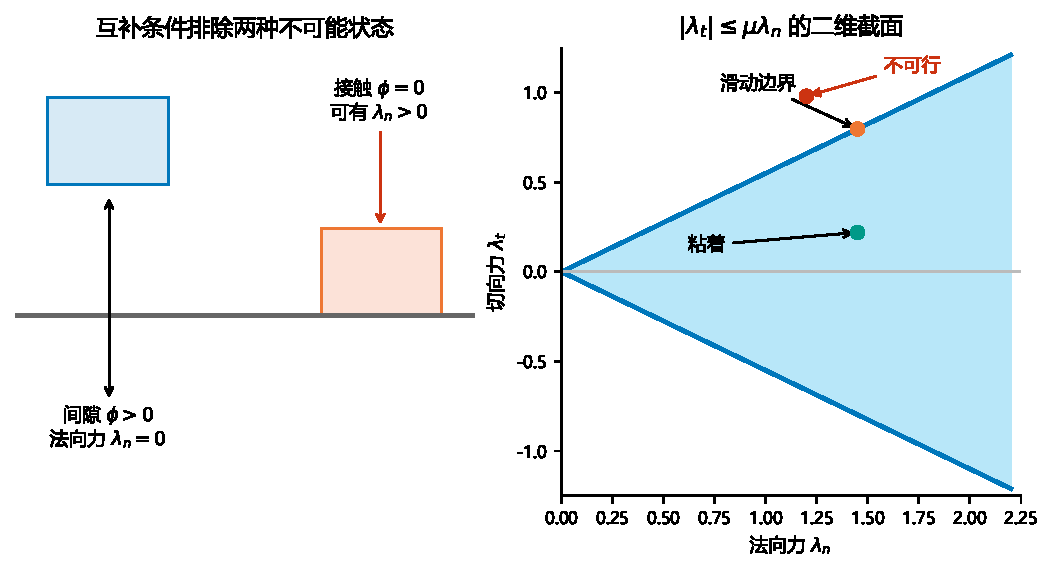
\includegraphics[width=\textwidth]{v0.3-06-接触互补与摩擦锥.pdf}
\caption{法向互补的合法/非法状态与库仑摩擦锥截面。作者依据刚性接触模型绘制；图为概念解释，不是实验数据\cite{featherstone2008rigid,lynch2017modern}。}
\label{fig:contact-complementarity-friction}
\end{figure}

接触建立或断开会改变约束集合，碰撞还会使速度发生跃迁。因此接触操作是混合系统：连续阶段用式\eqref{eq:joint-dynamics}演化，离散事件更新接触模式或施加冲量。柔顺材料和有限采样控制器常用罚函数 $\lambda_n=k_p[-\phi]_++d_p[-\dot\phi]_+$ 近似接触；它容易实现，却把允许穿透量、刚度和积分步长绑定在一起。减小步长并不自动消除模型偏差，增大刚度也可能造成数值发散。

\begin{table}[H]
\centering
\caption{接触建模选择及其代价}
\label{tab:contact-models}
\begin{tabularx}{\textwidth}{p{0.18\textwidth}YYY}
\toprule
方法 & 主要变量 & 优点 & 典型失效\\
\midrule
刚性互补 & 间隙、接触力/冲量 & 不允许静态穿透，接触逻辑明确 & 求解不光滑，多接触时计算昂贵\\
罚函数 & 穿透量、相对速度 & 易并入常微分方程和自动微分 & 刚度与步长耦合，参数缺乏真实对应\\
可变形接触 & 形变场或局部材料参数 & 能表示软物体和接触斑 & 参数多，识别与实时计算困难\\
数据驱动残差 & 解析模型加学习修正 & 可补偿稳定的系统误差 & 外推不可控，不能替代不可穿透约束\\
\bottomrule
\end{tabularx}
\end{table}

\section{从关节力矩到任务空间阻抗}

末端速度满足 $\dot x=J(q)\dot q$。忽略奇异点并选定任务子空间后，操作空间惯量为
\begin{equation}
\Lambda(q)=\left(JM^{-1}J^\top\right)^{-1}.
\label{eq:operational-inertia}
\end{equation}
$\Lambda$ 说明同一笛卡尔方向在不同姿态呈现不同“等效质量”。若希望位姿误差 $e=x-x_d$ 在外力 $F_{ext}$ 下满足
\begin{equation}
M_d\ddot e+D_d\dot e+K_de=F_{ext},
\label{eq:desired-impedance}
\end{equation}
则最简任务空间弹簧--阻尼力为 $F_c=-K_de-D_d\dot e$，再经 $\tau=J^\top F_c+C\dot q+g$ 映射到关节。完整的操作空间控制还应补偿 $\Lambda$、任务空间科氏/重力项，并处理零空间任务\cite{khatib1987operational}。

式\eqref{eq:operational-inertia}可以从关节加速度关系看出。暂忽略 $\dot J\dot q$、重力和科氏项，若关节力矩由任务力产生，$\tau=J^\top F$，则 $\ddot x=JM^{-1}J^\top F=\Lambda^{-1}F$，因此 $F=\Lambda\ddot x$。当 $J$ 行满秩时该逆存在；接近奇异位形时，某些方向的等效惯量会急剧增大，直接求逆放大噪声。工程实现通常采用阻尼伪逆、限制任务方向或避开奇异区，而不是假定公式在所有构型都数值良好。

阻抗控制给定位移到力的映射；导纳控制则测量外力，再由虚拟动力学积分得到位置或速度命令。高带宽力矩接口常适合外环阻抗，只有位置接口的工业机械臂更常用导纳外环。两者的稳定性都受环境刚度、采样延迟和内环动态影响\cite{deschutter1997force}。“把 $K_d$ 调低就安全”并不成立：过软会造成定位误差和长时间摩擦，过低阻尼会在接触切换时振荡。

\begin{figure}[H]
\centering
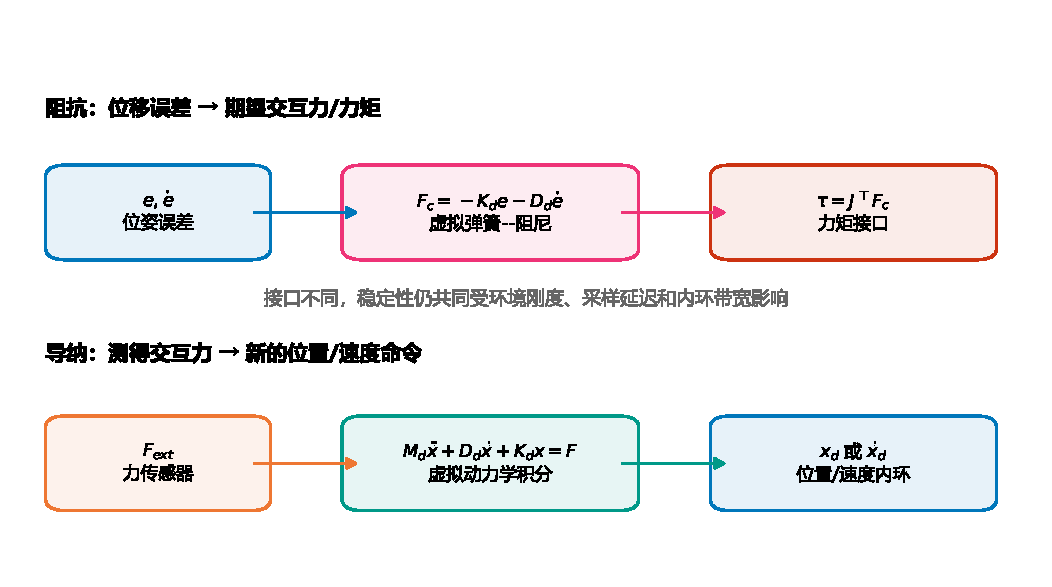
\includegraphics[width=\textwidth]{v0.3-06-阻抗与导纳接口.pdf}
\caption{阻抗与导纳的信号方向和执行器接口。作者依据经典力控制分类绘制\cite{hogan1985impedance,deschutter1997force}。}
\label{fig:impedance-admittance-interface}
\end{figure}

图\ref{fig:impedance-admittance-interface}中的差别决定代码落点。阻抗外环从位置/速度误差计算期望交互力或关节力矩，依赖可控力矩接口；导纳外环从测得外力积分出新的位置/速度命令，可包在厂商位置伺服器之外。后者并不天然更稳定：力传感噪声会被积分，位置内环延迟又会改变虚拟质量、阻尼和环境刚度组成的闭环极点。

\subsection{一维参数算例}

设期望接触方向的虚拟质量 $m_d=2\ \mathrm{kg}$、刚度 $k_d=800\ \mathrm{N/m}$。临界阻尼为 $d_d=2\sqrt{m_dk_d}=80\ \mathrm{N\,s/m}$，固有频率 $\omega_n=\sqrt{k_d/m_d}=20\ \mathrm{rad/s}$。若环境位置误差为 $2\ \mathrm{mm}$，静态弹簧力约为 $1.6\ \mathrm{N}$；若标定误差增至 $10\ \mathrm{mm}$，则为 $8\ \mathrm{N}$。控制律没有改变，但几何误差把交互力放大了五倍。这就是为什么接触控制章节必须同时讨论标定、阈值和回退。

\section{官方实现导读：方程如何落到实时回调}

libfranka 0.15.0 的官方示例在 1 个实时回调中读取科氏项、末端雅可比和关节速度，构造弹簧--阻尼任务力矩，并把科氏补偿相加\cite{libfranka015}。以下片段保留其关键计算，省略连接、姿态误差和异常处理：

\begin{lstlisting}[language=C++,caption={libfranka 0.15.0 笛卡尔阻抗示例的关键力矩计算（Apache-2.0）}]
auto coriolis_array = model.coriolis(robot_state);
auto jacobian_array = model.zeroJacobian(
    franka::Frame::kEndEffector, robot_state);
Eigen::Map<const Eigen::Matrix<double, 7, 1>>
    coriolis(coriolis_array.data());
Eigen::Map<const Eigen::Matrix<double, 6, 7>>
    jacobian(jacobian_array.data());
Eigen::Map<const Eigen::Matrix<double, 7, 1>>
    dq(robot_state.dq.data());
tau_task = jacobian.transpose()
         * (-stiffness * error - damping * (jacobian * dq));
tau_d = tau_task + coriolis;
\end{lstlisting}
\sourceanchor{仓库 \texttt{frankarobotics/libfranka}；tag \texttt{0.15.0}；文件 \texttt{examples/cartesian\_impedance\_control.cpp}；许可证 Apache-2.0；符号 \texttt{impedance\_control\_callback}。}

代码与式\eqref{eq:desired-impedance}之间存在三个值得检查的差异。第一，示例明确“不做惯量整形”，所以 $M_d$ 不是任意指定的常数矩阵；实际闭环惯量随构型变化。第二，示例的旋转误差由四元数构造，不能把欧氏角度误差原样复制。第三，官方文档警告该示例把碰撞阈值设得较高，并要求操作者握住急停。示例能解释算法，不等于通过生产安全验证。

\section{完整案例：带搜索与回退的柔顺插装}

考虑圆柱销插入孔。已知末端标称孔位 $\hat x_h$，但横向误差可能达到 $\pm2\ \mathrm{mm}$；六维力/力矩传感器提供 $w=[f_x,f_y,f_z,m_x,m_y,m_z]$。任务不是“沿 $z$ 轴下降”，而是一个带观测判据的状态机：

\begin{figure}[H]
\centering
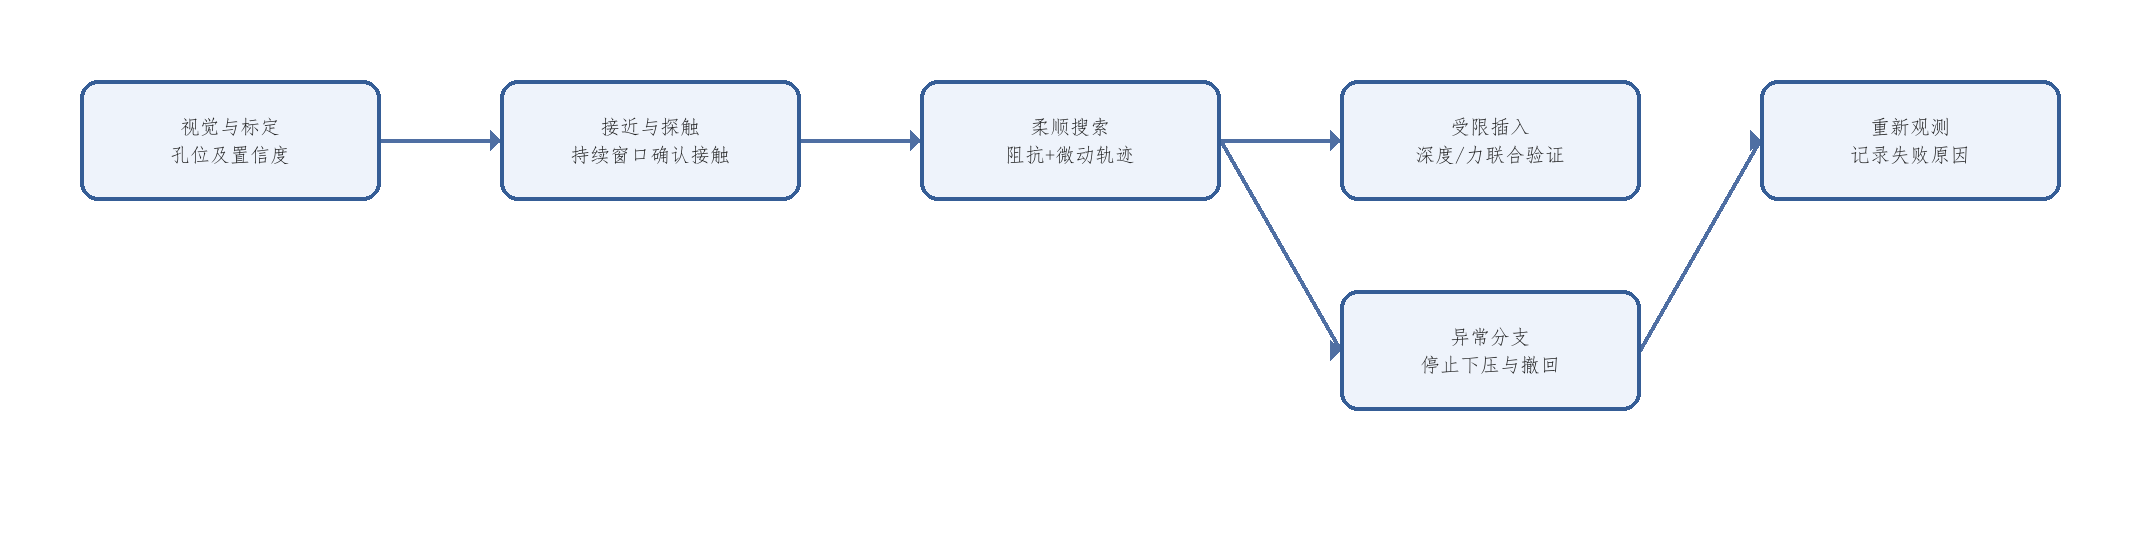
\includegraphics[width=\textwidth]{v0.3-06-柔顺插装闭环.png}
\caption{柔顺插装的观测、控制与异常恢复链。作者自绘；概念依据为阻抗/力控制文献\cite{hogan1985impedance,deschutter1997force}，不复制论文原图。}
\label{fig:compliant-insertion-loop}
\end{figure}

\begin{enumerate}
  \item \textbf{接近：}在自由空间移动到孔上方，限制速度和动能；检查视觉置信度、工具标定版本和工件是否到位。
  \item \textbf{探触：}沿 $-z$ 低速移动。当 $f_z>f_{contact}$ 持续 $N$ 个采样周期时确认接触，避免单点噪声触发。
  \item \textbf{搜索：}保持法向期望力或低法向刚度，在 $xy$ 平面执行螺旋/栅格微动；横向力和力矩用于判断卡边。
  \item \textbf{插入：}检测到 $z$ 位移增加且横向力下降后，切换到较高横向刚度和受限轴向速度。
  \item \textbf{验证：}以深度、末端残余力和工件存在信号共同判定成功；单一位置阈值可能把工件变形误判为到位。
  \item \textbf{回退：}若 $\|f_{xy}\|>f_{jam}$、$|m_{xy}|>m_{jam}$ 或搜索超时，立即停止下压，沿已知安全方向撤回，重新观测孔位；重复次数超过上限则转人工。
\end{enumerate}

\begin{lstlisting}[language=Python,caption={教学伪代码：插装状态机；非任何厂商源码}]
while not terminal:
    wrench = low_pass(read_wrench())
    if state == APPROACH:
        command_pose(pre_insert)
    elif state == TOUCH and persistent(wrench.fz > f_contact, N):
        state = SEARCH
    elif state == SEARCH:
        command_impedance(spiral_xy(), vz=-v_probe, K=K_search)
        if insertion_signature(depth, wrench): state = INSERT
        if jam(wrench) or timeout(): state = RETRACT
    elif state == RETRACT:
        stop_downward_motion(); retract(); reacquire_hole()
\end{lstlisting}

这段伪代码故意把控制命令与判据分开。$f_{contact}$、$f_{jam}$ 和滤波窗口不能凭经验永久写死：它们需要由传感器噪声、正常接触分布、工件公差和允许风险共同标定。部署日志至少应保存原始/滤波力、位姿、状态转换原因、控制器参数和失败图像，否则失败样本无法回流到几何估计或策略训练。

\section{知识小结与综述判断}

\textbf{知识小结。}关节空间动力学把执行器力矩、惯性、科氏/离心、重力和接触广义力置于同一方程；单边接触由间隙、法向力和互补条件描述，摩擦锥区分粘着与滑动；任务空间惯量说明末端方向上的动态响应随构型变化；阻抗与导纳控制分别规定运动--力关系及力到运动的外环映射。柔顺插装需要状态机、阈值和恢复链，不能只给出一条控制方程。

\authorjudgement{经典阻抗和操作空间理论仍是接触操作的主干，不是等待被 VLA 淘汰的“传统模块”。学习策略最有价值的切入点通常是难以建模的搜索轨迹、接触状态估计和参数调节；安全力限、实时内环、急停与确定性回退仍应由可验证的控制层承担。若一项工作只报告成功率而不报告接触力、超时、卡死和人工恢复，它不足以证明接触操作能力。}


\chapter[运动规划、轨迹优化与最优控制]{运动规划、轨迹优化\\与最优控制}
\label{chap:planning-optimal-control}

\section{学习目标、前置知识与问题边界}

本章把“机器人怎样到达目标”拆成三个不同问题。运动规划寻找不碰撞的几何路径；轨迹生成给路径加上时间、速度和加速度；反馈控制在模型误差与扰动下持续修正执行。读完本章，读者应能写出三者各自的决策变量和约束，推导有限时域 LQR 的反向递推，解释轨迹优化与 MPC 的联系，并为一个受约束任务选择可验证的组合，而不是把 A*、RRT、LQR 与 MPC 当作并列名词。

前置知识是第~\ref{chap:math-computation}章的约束优化、第~\ref{chap:kinematics-lie}章的构型与雅可比，以及第~\ref{chap:dynamics-contact-compliance}章的动力学。高层任务规划和 VLA 只向本章提供目标、代价或参考轨迹；它们不能替代碰撞约束、执行器边界和毫秒级反馈。

\begin{figure}[H]
\centering
\setlength{\tabcolsep}{5pt}
\begin{tabular}{c@{\ $\longrightarrow$\ }c@{\ $\longrightarrow$\ }c}
\fbox{\begin{minipage}{0.25\textwidth}\centering 几何路径\\$q(s)\in\mathcal C_{\mathrm{free}}$\\不含时间\end{minipage}} &
\fbox{\begin{minipage}{0.25\textwidth}\centering 带时轨迹\\$q(t),\dot q(t),\ddot q(t)$\\满足运动边界\end{minipage}} &
\fbox{\begin{minipage}{0.25\textwidth}\centering 闭环控制\\$u_t=\pi(x_t,r_t)$\\抵抗扰动\end{minipage}}
\end{tabular}
\caption{从几何可行到动态可执行的三层接口。作者教学绘制；箭头表示上游结果成为下游参考，不表示一次求解即可完成任务。}
\label{fig:path-trajectory-feedback}
\end{figure}

\section{构型空间、碰撞与采样规划}

令机器人构型为 $q\in\mathcal C$，碰撞构型集合为 $\mathcal C_{\mathrm{obs}}$，则自由空间为 $\mathcal C_{\mathrm{free}}=\mathcal C\setminus\mathcal C_{\mathrm{obs}}$。几何规划寻找连续曲线
\begin{equation}
q:[0,1]\rightarrow\mathcal C_{\mathrm{free}},\qquad q(0)=q_s,\quad q(1)\in\mathcal Q_g.
\label{eq:geometric-path}
\end{equation}
这里的碰撞检查不是图形显示功能，而是可行性判定器。机械臂的一个末端位姿通常对应多个关节构型；只在笛卡尔空间画直线，既可能穿过障碍，也可能越过关节限位或奇异区。

离散栅格或低维图上可用 Dijkstra/A*；高维连续空间常用 PRM、RRT 及其变体。RRT 反复采样 $q_{\mathrm{rand}}$，从树中最近节点向样本延伸并做局部碰撞检查。它在常见条件下具有概率完备性：若存在具有正裕量的可行路径，样本数增加时找到路径的概率趋近于一；但原始 RRT 不保证路径代价趋近最优。RRT* 增加邻域选父与重连，使代价在相应假设下几乎必然趋近最优\cite{karaman2011sampling}。

“渐近最优”不等于有限时间最好。狭窄通道的有效体积很小，均匀采样可能长期碰不到入口；碰撞检测往往占据主要计算量；错误的机器人几何、膨胀半径或场景时间戳会让规划器对错误世界给出数学上正确的路径。因而应记录采样预算、碰撞模型版本、最小净空和终止原因，而不只记录“规划成功”。

\section{轨迹优化：从一条初值到约束局部解}

将轨迹离散为 $Q=(q_0,\ldots,q_N)$，典型目标为
\begin{equation}
\min_Q\;\underbrace{\frac12\sum_{k=0}^{N-1}\|q_{k+1}-q_k\|_W^2}_{\text{平滑/控制代价}}
+\alpha\underbrace{\sum_{k=0}^{N}c_{\mathrm{obs}}(q_k)}_{\text{障碍代价}},
\quad\text{s.t. }q_0=q_s,\;q_N\in\mathcal Q_g,\;g(Q)\le0.
\label{eq:trajectory-optimization}
\end{equation}
$W$ 决定不同关节和时间差分的尺度；$c_{\mathrm{obs}}$ 常由有符号距离场构造；$g$ 收纳关节、速度、加速度和任务约束。CHOMP 使用轨迹空间的平滑度量和障碍代价梯度更新整条轨迹\cite{ratliff2009chomp}；TrajOpt 把非凸问题逐次凸化，并强调连续时间碰撞检查，避免只检查离散路点而在两点之间穿越障碍\cite{schulman2014motion}。

式~\eqref{eq:trajectory-optimization} 是局部优化：初值位于障碍哪一侧，常决定最终同伦类。一个常用工程组合是先用采样规划给出拓扑上可行的粗路径，再由轨迹优化增加净空和平滑性，最后做时间参数化。若直接对一条穿障碍直线做梯度下降，距离场梯度在障碍内部可能不稳定，甚至把轨迹推入错误局部极小值。

路径参数 $s$ 与时间 $t$ 不能混用。给定 $q(s)$，有
\begin{equation}
\dot q=q'(s)\dot s,\qquad
\ddot q=q''(s)\dot s^2+q'(s)\ddot s.
\label{eq:time-parameterization}
\end{equation}
速度、加速度、力矩约束因此转化为对 $\dot s,\ddot s$ 的限制。简单地把相邻路点按固定周期发送给控制器，会在曲率大处产生速度/加速度跳变；几何无碰撞并不意味着动态可执行。

\section{LQR 与 DDP：为什么要反向传播一个二次值函数}

考虑线性离散系统 $x_{k+1}=A_kx_k+B_ku_k$，有限时域二次代价
\begin{equation}
J=x_N^\top Q_Nx_N+\sum_{k=0}^{N-1}
\left(x_k^\top Q_kx_k+u_k^\top R_ku_k\right),
\quad Q_k\succeq0,\;R_k\succ0.
\label{eq:lqr-cost}
\end{equation}
假设后续最优代价为 $V_{k+1}(x)=x^\top P_{k+1}x$，把动力学代入并对 $u_k$ 求极小，得到
\begin{align}
K_k&=(R_k+B_k^\top P_{k+1}B_k)^{-1}B_k^\top P_{k+1}A_k,\\
u_k^*&=-K_kx_k,\\
P_k&=Q_k+A_k^\top P_{k+1}A_k-A_k^\top P_{k+1}B_kK_k,
\quad P_N=Q_N.
\label{eq:riccati-recursion}
\end{align}
这不是凭经验选择反馈增益，而是动态规划下二次值函数的系数递推。$R$ 越大，控制动作越昂贵；$Q$ 越大，状态偏差越昂贵。二者量纲必须经缩放后再比较。

以标量系统 $x_{k+1}=x_k+u_k$、两步时域、$Q_0=Q_1=0$、$Q_2=1$、$R_0=R_1=1$ 为例。由 $P_2=1$ 得 $K_1=1/2,P_1=1/2$；再得 $K_0=(1+1/2)^{-1}(1/2)=1/3$。若 $x_0=3$，则 $u_0=-1,x_1=2$，随后 $u_1=-1,x_2=1$。有限时域和控制代价使系统不必在第一步把误差清零。

非线性系统可围绕名义轨迹线性化并反复执行上述反向/正向过程。iLQR/DDP 的核心是对动力学和代价作局部展开，再用线搜索接受新轨迹；控制受限 DDP 还在反向步显式处理动作边界\cite{tassa2014control}。它们仍是局部方法：接触模式突变、坏初值和不准确二阶近似都可能破坏收敛。

\section{MPC：把有限时域优化变成反馈}

模型预测控制在每个时刻求解
\begin{equation}
\begin{aligned}
\min_{x_{0:N},u_{0:N-1}}\quad&\ell_N(x_N)+\sum_{k=0}^{N-1}\ell(x_k,u_k)\\
\text{s.t.}\quad&x_{k+1}=f(x_k,u_k),\quad x_k\in\mathcal X,\quad u_k\in\mathcal U,\\
&x_0=\hat x_t,
\end{aligned}
\label{eq:mpc}
\end{equation}
只执行最优序列的第一个动作，收到新状态估计后平移时域并重算。与离线轨迹优化相比，MPC 通过重规划形成反馈，并可显式处理状态、动作与终端约束；其稳定性并非来自“每次都优化”这句话，而依赖终端代价/终端集合、递归可行性和模型假设\cite{mayne2000mpc}。

预测时域短会近视，时域长则增加求解时间和模型误差累积。若求解器超过控制周期，系统使用的是过期状态对应的动作；若约束突然不可行，必须有软约束、备份控制器或安全停车，而不能把上一次解无限复用。

\begin{lstlisting}[caption={滚动时域受约束控制的教学伪代码；非厂商或开源项目源码}]
while task_active:
    x_hat, stamp = estimator.latest()
    if now() - stamp > freshness_limit: safe_stop()
    problem.set_initial_state(x_hat)
    problem.set_reference(local_path, goal)
    sol = solver.solve(warm_start=shift(previous_sol))
    if not sol.feasible or sol.solve_time > deadline:
        execute(backup_controller(x_hat)); continue
    execute(rate_limit(sol.u[0]))
    previous_sol = sol
\end{lstlisting}

\section{同一受约束任务的接口比较}

设七轴机械臂要从货架外移动到箱内抓取位，场景有狭窄入口、关节速度/力矩限制和移动中的人。表~\ref{tab:planning-control-comparison} 的方法不是互斥竞品，而是处理不同变量与时间尺度。

\begin{table}[H]
\centering
\caption{同一任务中规划与控制方法的职责、证据与失效}
\label{tab:planning-control-comparison}
\begin{tabularx}{\textwidth}{p{0.15\textwidth}YYYY}
\toprule
方法 & 决策变量 & 主要约束/证据 & 是否反馈 & 典型失效 \\
\midrule
图搜索 & 离散节点路径 & 栅格连通与边代价 & 否 & 维数灾难、离散化漏障碍 \\
RRT/RRT* & 连续构型树 & 局部连接与碰撞检查 & 否 & 狭窄通道慢、有限预算路径差 \\
轨迹优化 & 整段路点/控制 & 距离场、平滑和边界 & 通常否 & 初值敏感、局部极小 \\
LQR/iLQR & 反馈增益/名义轨迹 & 局部动力学与二次代价 & 是 & 线性化失真、动作饱和 \\
MPC & 有限时域状态/动作 & 动力学、状态和动作集合 & 是 & 超时、不可行、模型偏差 \\
\bottomrule
\end{tabularx}
\end{table}

一个可审计组合是：RRT* 找到进入箱体的可行同伦类；轨迹优化提高净空并平滑；时间参数化满足速度/加速度边界；MPC 依据第~\ref{chap:state-estimation-slam}章的最新状态跟踪并避开动态障碍；第~\ref{chap:dynamics-contact-compliance}章的阻抗控制处理抓取前后的接触。若状态估计过期或动态障碍使问题不可行，系统退回保持位或安全撤离。这里每一层都有独立退出条件，因而能定位失败究竟发生在世界模型、几何可行性、动态可行性还是执行反馈。

\section{知识小结与综述判断}

知识小结：路径只描述构型随路径参数的变化，轨迹还包含时间导数，控制则把状态误差闭环到动作。采样规划擅长寻找非凸自由空间中的可行同伦类；轨迹优化擅长从初值改进平滑性和约束；LQR/DDP 用局部值函数得到反馈结构；MPC 以滚动时域把优化转成约束反馈。

综述判断：真实系统不应争论“规划还是学习”，而应明确学习模块输出的是目标、代价、初值、模型还是动作。只要机器人仍受碰撞、执行器和实时性约束，规划与控制的可行性检查就有独立价值；但它们的结论只对输入状态和模型有效，不能掩盖感知延迟、场景错误或接触建模缺失。

\chapter{状态估计、传感器融合与 SLAM}
\label{chap:state-estimation-slam}

\section{学习目标、前置知识与问题设定}

控制器读到的不是“真实状态”，而是由模型、传感器和时间戳共同生成的估计。读完本章，读者应能从贝叶斯递推推导卡尔曼预测与校正，解释 EKF、UKF、粒子滤波和因子图的假设差异，说明 SLAM 中位姿与地图为何耦合，并把时间同步、外参漂移与状态新鲜度写成可监控接口。

离散状态空间模型写为
\begin{equation}
x_k=f(x_{k-1},u_{k-1})+w_{k-1},\qquad
z_k=h(x_k)+v_k,
\label{eq:nonlinear-state-observation}
\end{equation}
$x_k$ 可含位姿、速度、IMU 偏置和地图路标，$z_k$ 是相机、雷达、编码器或力觉观测；$w,v$ 分别是过程和观测噪声。式中下标也是时间语义：若 $z_k$ 实际对应旧时刻却按当前状态融合，正确的矩阵运算仍会得到错误估计。

\begin{figure}[H]
\centering
\setlength{\tabcolsep}{3pt}
\begin{tabular}{c@{\ $\longrightarrow$\ }c@{\ $\longrightarrow$\ }c@{\ $\longrightarrow$\ }c}
\fbox{\begin{minipage}{0.17\textwidth}\centering 上一后验\\$\hat x^+,P^+$\end{minipage}} &
\fbox{\begin{minipage}{0.15\textwidth}\centering 模型预测\\$f,Q$\end{minipage}} &
\fbox{\begin{minipage}{0.17\textwidth}\centering 创新检验\\$r_k,S_k$\end{minipage}} &
\fbox{\begin{minipage}{0.17\textwidth}\centering 当前后验\\$\hat x^+,P^+$\\附时间戳\end{minipage}}
\end{tabular}
\caption{递归状态估计的数据流。作者教学绘制；创新门控与时间戳检查是估计器接口的一部分，不是日志附属项。}
\label{fig:state-estimation-loop}
\end{figure}

\section{线性高斯模型与卡尔曼滤波}

对线性模型
\begin{equation}
x_k=F_{k-1}x_{k-1}+B_{k-1}u_{k-1}+w_{k-1},\quad
z_k=H_kx_k+v_k,
\end{equation}
令 $w\sim\mathcal N(0,Q)$、$v\sim\mathcal N(0,R)$ 且相互独立。高斯分布经线性变换仍为高斯，因此预测为
\begin{align}
\hat x_{k|k-1}&=F_{k-1}\hat x_{k-1|k-1}+B_{k-1}u_{k-1},\\
P_{k|k-1}&=F_{k-1}P_{k-1|k-1}F_{k-1}^\top+Q_{k-1}.
\label{eq:kf-predict}
\end{align}
观测创新及其协方差为 $r_k=z_k-H_k\hat x_{k|k-1}$、$S_k=H_kP_{k|k-1}H_k^\top+R_k$。最小化更新后误差协方差可得\cite{kalman1960new}
\begin{align}
K_k&=P_{k|k-1}H_k^\top S_k^{-1},\\
\hat x_{k|k}&=\hat x_{k|k-1}+K_kr_k,\\
P_{k|k}&=(I-K_kH_k)P_{k|k-1}.
\label{eq:kf-update}
\end{align}
$K_k$ 不是人工信任系数，而是先验不确定性与观测不确定性的矩阵权衡。数值实现宜使用线性求解代替显式 $S^{-1}$，并可用 Joseph 形式
\begin{equation}
P_{k|k}=(I-KH)P^-(I-KH)^\top+KRK^\top
\end{equation}
减轻有限精度造成的非对称或非正定。

一维算例最能说明增益含义。先验位置为 $8\ \mathrm m$、方差 $P^-=4\ \mathrm{m^2}$；测量为 $9\ \mathrm m$、方差 $R=1\ \mathrm{m^2}$，且 $H=1$。则 $K=4/(4+1)=0.8$，后验 $\hat x^+=8+0.8(9-8)=8.8\ \mathrm m$，方差 $P^+=(1-0.8)4=0.8\ \mathrm{m^2}$。若把测量方差错写成 $0.01$，滤波器会几乎完全追随传感器；这不是“融合更灵敏”，而是噪声模型失配。

可观测性决定观测序列能否区分内部状态。线性时不变系统的可观测矩阵
\begin{equation}
\mathcal O=\begin{bmatrix}H^\top&(HF)^\top&\cdots&(HF^{n-1})^\top\end{bmatrix}^\top
\end{equation}
须满列秩才能从有限序列重构全部状态。滤波器能输出一个数，不代表该状态可观；不可观方向的协方差若被错误压小，会形成危险的“自信漂移”。

\section{非线性滤波：线性化、sigma 点与样本}

EKF 在当前估计附近以雅可比 $F_k=\partial f/\partial x$、$H_k=\partial h/\partial x$ 线性化，再使用式~\eqref{eq:kf-predict}--\eqref{eq:kf-update}。它计算紧凑，但线性化点错误、姿态参数化不连续或强非线性会造成不一致。误差状态滤波把姿态等流形状态保留在名义值上，只在切空间估计小误差；第~\ref{chap:kinematics-lie}章的 $SO(3)/SE(3)$ 正是为此提供接口\cite{sola2017quaternion,barfoot2024state}。

UKF 选取一组确定性 sigma 点，使其样本均值与协方差匹配当前高斯分布；每个点通过非线性 $f,h$ 后重新加权均值与协方差，从而避免显式雅可比\cite{julier2004ukf}。它并没有消除高斯假设，也不能自动处理多峰后验。粒子滤波则用带权样本近似后验，可表示多峰和强非线性，但维数升高时需要大量粒子，重采样还会造成样本贫化。

\begin{table}[H]
\centering
\caption{递归估计与批量平滑方法的假设和失效}
\label{tab:estimators-comparison}
\begin{tabularx}{\textwidth}{p{0.14\textwidth}YYYY}
\toprule
方法 & 后验表示 & 非线性处理 & 主要优势 & 典型失效 \\
\midrule
KF & 单高斯 & 线性模型 & 闭式、快速、可解释 & 模型或噪声非线性/非高斯 \\
EKF & 局部高斯 & 一阶雅可比 & 适合高频惯导融合 & 线性化不一致、雅可比错误 \\
UKF & 单高斯 & sigma 点传播 & 无需显式雅可比 & 高维点数增加、仍是单峰 \\
粒子滤波 & 带权样本 & 直接采样传播 & 可表示多峰 & 维数灾难、样本贫化 \\
因子图平滑 & 轨迹联合分布 & 非线性最小二乘 & 可重线性化、用回环修正历史 & 内存/求解开销、错误数据关联 \\
\bottomrule
\end{tabularx}
\end{table}

创新 $r_k$ 是最直接的在线诊断量。若模型正确，归一化创新平方 $r_k^\top S_k^{-1}r_k$ 应与观测维数对应的 $\chi^2$ 分布大致一致。长期偏大表示 $Q/R$ 太小、模型遗漏或观测异常；长期偏小可能表示协方差过于保守。门控只能拒绝离群值，不能修复持续偏置和错误外参。

\section{从递归滤波到因子图与 SLAM}

SLAM 同时估计机器人轨迹 $X=(x_0,\ldots,x_T)$ 与地图 $M$。里程计约束把相邻位姿连接，路标观测把位姿与地图点连接，回环约束把远隔时刻重新连接。定位依赖地图，地图又由带不确定性的位姿观测生成，因此二者不能作为独立黑盒串联\cite{durrantwhyte2006slam}。

在独立高斯测量下，最大后验估计可写成非线性最小二乘
\begin{equation}
X^*=\arg\min_X\sum_i\|r_i(X_i)\|_{\Sigma_i^{-1}}^2,
\label{eq:factor-graph-objective}
\end{equation}
每个因子只依赖少量变量，雅可比和正规方程因此稀疏。批量平滑会重新优化整个窗口；固定滞后平滑只保留最近状态；iSAM2 用 Bayes tree 对受新因子影响的部分增量重线性化和重求解\cite{kaess2012isam2}。相较只保留当前后验的滤波，平滑能让回环观测修正历史轨迹，但计算和内存代价更高。

视觉 SLAM 的典型管线包括特征/直接跟踪、局部地图、关键帧优化、回环检测与全局图优化。ORB-SLAM2 用统一系统覆盖单目、双目和 RGB-D 相机，并公开了关键帧式实现\cite{murartal2017orbslam2}。这类系统的公开精度不能直接迁移到另一相机、镜头、曝光和运动模式：低纹理、重复纹理、运动模糊、动态物体和时间不同步都会改变数据关联质量。

地图也不是单一对象。占据栅格回答哪里可通行，稠密几何回答表面形状，语义地图记录对象与区域，拓扑图记录地点连通。面向移动操作时，控制器通常需要带协方差和时间戳的局部位姿/速度，规划器需要碰撞几何，高层任务需要对象语义；强迫一个地图同时承担全部职责，会把更新频率、坐标系和不确定性混在一起。

\section{时间同步、外参与状态新鲜度}

设机器人以速度 $v$ 运动，传感器时间偏差为 $\Delta t$，则仅时间错位就产生约 $\|v\|\Delta t$ 的位置误差；旋转角速度 $\omega$ 产生约 $\|\omega\|\Delta t$ 的姿态误差。以 $v=1.5\ \mathrm{m/s}$、$\Delta t=80\ \mathrm{ms}$ 为例，位置错位为 $0.12\ \mathrm m$。若规划器的安全净空只有 $0.10\ \mathrm m$，再准确的几何地图也无法补偿这段时间误差。

外参把传感器坐标系变到机体或世界系。相机支架松动造成的 $1^\circ$ 姿态漂移，在 $5\ \mathrm m$ 距离上对应约 $8.7\ \mathrm{cm}$ 的横向误差。若只调大观测噪声，滤波器可能表现得更平滑，却不会消除系统偏置。工程上应把时间偏差、外参和 IMU 偏置视为可标定/可估计状态，并监控它们的可观测条件。

\begin{lstlisting}[caption={带时间戳、创新门控和新鲜度检查的融合教学伪代码}]
for measurement in time_ordered_queue:
    predict_to(measurement.stamp, imu_buffer)
    residual, S = innovation(measurement)
    if residual.T @ solve(S, residual) > chi2_gate:
        reject(measurement); continue
    update(measurement)
    enforce_symmetric_positive_covariance()

state, stamp = estimator.latest()
if now() - stamp > control_freshness_limit:
    controller.enter_safe_hold()
\end{lstlisting}

该伪代码刻意把“融合”和“向控制器发布”分开：估计器即使仍在运行，也可能因队列堵塞发布过期状态。除均值和协方差外，状态包至少应携带参考坐标系、测量时间、发布时间、外参版本、有效性标志和最近一次拒绝/重定位原因。

\section{移动操作案例：误差如何沿系统栈传播}

考虑移动底盘把机械臂送到货架前抓取。底盘定位使用轮速、IMU 和视觉，机械臂末端又依赖底盘到世界的变换。若视觉延迟导致底盘横向位姿偏差 $12\ \mathrm{cm}$，局部规划器可能仍在旧坐标系中认为通道有净空；机械臂到位后，末端相对货架的同量级偏差会触发第~\ref{chap:dynamics-contact-compliance}章的异常接触。此时提高阻抗控制器柔顺性只能降低冲击，不能恢复错误几何。

可验证的回退链为：首先用创新统计和传感器心跳区分离群观测与数据中断；其次检查状态时间戳和外参版本；若协方差或新鲜度越界，停止进入狭窄区并退到已知安全位；只有在局部重定位或重新标定后，才让第~\ref{chap:planning-optimal-control}章的规划器基于新地图重算。日志需保留原始时间戳、接受/拒绝原因、状态协方差、规划版本和最终动作，否则无法判断失败源于估计、规划还是控制。

\section{知识小结与综述判断}

知识小结：状态估计是带模型和不确定性的时间递推。KF 对线性高斯模型给出闭式预测/校正；EKF 用局部雅可比，UKF 用 sigma 点，粒子滤波用样本；因子图把整段轨迹写成稀疏最小二乘，使回环能修正历史。SLAM 的地图、位姿、数据关联和坐标系是一体化估计问题。

综述判断：具身系统最常见的估计风险不是“算法不够新”，而是时间、坐标系、偏置和协方差口径没有成为接口契约。后续的世界模型和长期记忆可以增加语义，但只要动作要落到真实身体，控制器仍需要一个带时间戳、参考系和可信度的物理状态；没有这些元数据，模型输出再丰富也无法形成可审计闭环。

\chapter{模仿学习、DAgger 与偏好学习}
\label{chap:imitation-preference}

\section{问题设定：学习动作，还是学习目标}

示教数据通常写为 $\mathcal D_E=\{(o_t,a_t^E)\}$。行为克隆直接学习 $\pi_\theta(a\mid o)$；逆强化学习和偏好学习则先从轨迹比较中恢复奖励或效用，再由规划或强化学习求策略。二者回答不同问题：前者问“专家在这个观测下做了什么”，后者问“哪些结果更符合人的意图”。本章只讨论示教与偏好数据如何形成监督信号；MDP 与策略优化留给第~\ref{chap:reinforcement-learning}章，生成式动作分布留给第~\ref{chap:generative-action-policy}章。

\begin{figure}[H]
\centering
\begin{tabular}{c@{\ $\rightarrow$\ }c@{\ $\rightarrow$\ }c@{\ $\rightarrow$\ }c}
\fbox{专家/接管} & \fbox{轨迹与偏好} & \fbox{策略或奖励模型} & \fbox{影子评估与回流}
\end{tabular}
\caption{示教学习的闭环。作者教学绘制；关键不是一次性收集“干净数据”，而是明确哪些状态由当前策略访问、哪些失败需要重新标注。}
\label{fig:imitation-data-loop}
\end{figure}

\section{行为克隆与协变量偏移}

离散动作的行为克隆最小化负对数似然
\begin{equation}
\mathcal L_{\mathrm{BC}}(\theta)
=-\frac1N\sum_{i=1}^{N}\log\pi_\theta(a_i^E\mid o_i),
\label{eq:bc-nll}
\end{equation}
连续确定性动作常用 $\|a_i^E-\mu_\theta(o_i)\|_2^2$。这相当于假设给定观测只有一个条件均值；当“从杯子左侧绕过”和“从右侧绕过”都正确时，均方误差可能预测两条路线的平均值，恰好撞向杯子。第~\ref{chap:generative-action-policy}章将用动作块与生成模型处理这种多峰性。

更根本的问题是训练状态来自专家分布 $d_{\pi_E}$，部署状态来自学习策略自己的分布 $d_{\pi_\theta}$。一次小误差会把机器人带到示教中未出现的状态，后续预测因此更差。若把每一步独立失误率粗略写成 $\epsilon$，长度为 $T$ 的执行至少一次失误概率为 $1-(1-\epsilon)^T$。取 $\epsilon=0.02,T=50$，该概率约为 $63.6\%$；这不是严格的 DAgger 理论界，但直观说明逐帧准确率不能代替长时域成功率。

行为克隆仍是强基线：数据充足、闭环稳定、任务短且训练与部署分布接近时，它避免在线试错并易于调试。合格实验应同时报告轨迹级成功、恢复成功、接管次数、失败状态覆盖和动作延迟，而不只报告验证集 MSE。

\section{DAgger：在策略访问的状态上重新提问}

DAgger 迭代执行当前策略，收集其访问状态，并请求专家对这些状态给出动作，然后聚合到训练集\cite{ross2011dagger}。第 $i$ 轮可写为
\begin{equation}
\pi_i=\operatorname{Train}(\mathcal D_i),\qquad
\mathcal D_{i+1}=\mathcal D_i\cup
\{(o,a^E(o)):o\sim d_{\tilde\pi_i}\},
\end{equation}
其中 $\tilde\pi_i$ 可按概率混合专家与学习策略。它修正的不是模型容量，而是监督数据与部署状态分布的错位。

\begin{lstlisting}[caption={带安全接管和聚合预算的 DAgger 教学伪代码}]
dataset = expert_demonstrations
for round in range(max_rounds):
    policy = train_bc(dataset)
    for episode in shadow_or_guarded_rollouts(policy):
        for observation in episode:
            if supervisor.unsafe(observation):
                expert_action = supervisor.take_over(observation)
                dataset.add(observation, expert_action,
                            reason="safety_intervention")
    stop_if(validation_success_stable and intervention_rate_low)
\end{lstlisting}

真机 DAgger 的代价常被低估。专家必须在偏离状态下给出有意义动作；人机切换有延迟；“专家动作”可能依赖操作者看得到、策略看不到的信息；主动探索还可能损坏设备。因此工程实现常采用影子模式、仿真扰动、人工回放标注或只在安全域内聚合，而不是无条件让未成熟策略自由运行。

\section{逆强化学习与偏好学习}

逆强化学习假设专家行为近似优化某个未知奖励 $r_\phi(s,a)$。经典学徒学习通过匹配专家与策略的特征期望寻找奖励和策略\cite{abbeel2004apprenticeship}。奖励并不唯一：对所有轨迹加常数，甚至作势函数变换，都可能保持最优策略不变。因而恢复到的是与行为等价的一类目标，而不是专家脑中的“真实动机”。

偏好学习让标注者比较两段轨迹 $\tau^A,\tau^B$。若段得分为 $R_\phi(\tau)=\sum_t r_\phi(s_t,a_t)$，Bradley--Terry 模型给出
\begin{equation}
P_\phi(\tau^A\succ\tau^B)
=\frac{\exp R_\phi(\tau^A)}{\exp R_\phi(\tau^A)+\exp R_\phi(\tau^B)}.
\label{eq:preference-probability}
\end{equation}
对人类标签做交叉熵即可训练奖励模型，再用它优化策略。Christiano 等展示了从少量轨迹片段比较学习复杂目标的路径\cite{christiano2017preferences}。但奖励模型会被策略主动寻找漏洞；标注者间分歧、比较顺序、视频视角和未显示的安全信息都会进入标签噪声。

\begin{table}[H]
\centering
\caption{示教与偏好路线的监督对象和主要风险}
\label{tab:imitation-preference-comparison}
\begin{tabularx}{\textwidth}{p{0.15\textwidth}YYYY}
\toprule
方法 & 监督信号 & 是否需在线访问 & 优点 & 典型失效 \\
\midrule
行为克隆 & 状态--动作对 & 否 & 简单、稳定、可离线训练 & 协变量偏移、多峰平均 \\
DAgger & 当前策略状态上的专家动作 & 是/受控 & 直接覆盖恢复状态 & 标注昂贵、接管延迟 \\
逆强化学习 & 专家轨迹 & 常需反复求策略 & 可迁移目标表述 & 奖励不可辨识、计算昂贵 \\
偏好奖励 & 轨迹片段成对排序 & 可离线或主动查询 & 不要求逐帧动作 & 标注分歧、奖励黑客 \\
\bottomrule
\end{tabularx}
\end{table}

\section{示教策略上线：从数据到失败回流}

一个可审计流程包含五个门。第一，采集时保存原始观测、动作、操作者、设备标定、时间戳和任务结果；第二，按场景和操作者划分训练/验证集，避免相邻帧泄漏；第三，影子评估只记录策略建议，不驱动执行器；第四，在低速、限空间和人工接管下灰度；第五，把失败按感知、动作、时延、接触和任务定义分类后回流。只把成功轨迹追加到数据集，会系统性删除恢复行为。

上线指标应区分离线拟合与闭环结果。动作误差可发现单位或坐标问题，轨迹成功率衡量任务完成，接管率反映安全负担，失败恢复率衡量是否能离开分布外状态。任何指标都要按任务难度、物体和环境切片；总体平均数可能掩盖某个高风险子域完全失败。

\section{知识小结与综述判断}

知识小结：行为克隆在专家分布上做监督学习；DAgger 把监督查询移到当前策略访问的状态；逆强化学习和偏好学习把人类行为转成奖励或效用。四者的关键差异是标注对象、数据分布和是否允许在线访问，而不是网络骨干。

综述判断：机器人示教系统的上限常由数据协议而非损失函数决定。若观测不含专家决策所需信息、失败状态从不标注、接管延迟不记录，再复杂的策略也只能拟合一个不可部署的数据集。评价应把知识讲解与上线证据分开：先说明算法在什么假设下成立，再报告真实闭环是否满足这些假设。

\chapter{强化学习：从 MDP 到离线与安全 RL}
\label{chap:reinforcement-learning}

\section{MDP 是交互假设，不是算法名称}

马尔可夫决策过程写为 $\mathcal M=(\mathcal S,\mathcal A,P,r,\gamma)$。策略 $\pi(a\mid s)$ 产生动作，环境按 $P(s'\mid s,a)$ 转移并给奖励 $r$。目标是最大化
\begin{equation}
J(\pi)=\mathbb E_{\tau\sim\pi}\left[\sum_{t=0}^{T}\gamma^t r(s_t,a_t)\right].
\label{eq:rl-objective}
\end{equation}
“状态”必须足以预测未来；若相机图像缺少速度、接触历史或目标身份，实际问题是部分可观测的。第~\ref{chap:state-estimation-slam}章提供物理状态估计，第~\ref{chap:representation-transfer}章讨论学习表示，本章只研究给定状态/历史后怎样优化长期回报。

\begin{figure}[H]
\centering
\begin{tabular}{c@{\ $\rightarrow$\ }c@{\ $\rightarrow$\ }c@{\ $\rightarrow$\ }c}
\fbox{策略 $\pi$} & \fbox{动作 $a_t$} & \fbox{环境 $P$} & \fbox{状态与奖励 $s_{t+1},r_t$}
\end{tabular}
\caption{在线强化学习的数据闭环。作者教学绘制；离线 RL 切断了策略到环境的新交互箭头，只能使用固定日志。}
\label{fig:rl-interaction-loop}
\end{figure}

\section{价值函数、Bellman 方程与策略梯度}

策略价值和动作价值为
\begin{align}
V^\pi(s)&=\mathbb E_\pi\left[\sum_{k=0}^{\infty}\gamma^k r_{t+k}\mid s_t=s\right],\\
Q^\pi(s,a)&=\mathbb E_\pi\left[\sum_{k=0}^{\infty}\gamma^k r_{t+k}\mid s_t=s,a_t=a\right].
\end{align}
按第一步拆分得到 Bellman 期望方程
\begin{equation}
Q^\pi(s,a)=r(s,a)+\gamma\,
\mathbb E_{s'\sim P,a'\sim\pi}[Q^\pi(s',a')].
\label{eq:bellman-expectation}
\end{equation}
它把长时域目标转成一步奖励加后继价值，但也把模型、奖励和价值估计误差递归传播\cite{sutton2018reinforcement}。

以确定性两状态任务为例：在 $s_0$ 执行动作后即时奖励 1 并到 $s_1$，$s_1$ 的后续价值为 5，$\gamma=0.9$，则 $Q(s_0,a)=1+0.9\times5=5.5$，不是即时奖励 1。若价值 5 来自分布外动作的过估计，错误也被折扣后写回 $s_0$。

对可微随机策略，策略梯度定理给出
\begin{equation}
\nabla_\theta J(\pi_\theta)
=\mathbb E_{s,a\sim\pi_\theta}
\left[\nabla_\theta\log\pi_\theta(a\mid s)A^\pi(s,a)\right],
\label{eq:policy-gradient}
\end{equation}
$A=Q-V$ 衡量动作相对基线的增益。actor--critic 用 actor 表示策略、critic 估计 $V$ 或 $Q$。基线降低方差但不消除偏差；critic 错误会直接误导 actor。

最大熵方法在奖励之外鼓励策略熵。Soft Actor-Critic 使用离策略数据和熵正则，在连续控制中兼顾探索与样本复用\cite{haarnoja2018sac}。熵系数不是“随机程度旋钮”这么简单：动作维度、缩放和执行器饱和都会改变实际探索能量。

\section{在线、离线与示教增强：数据假设的差别}

在线 RL 可以用当前策略收集新数据并纠正价值估计，但真机样本昂贵且探索危险。离策略在线方法可复用旧数据，但仍假设能继续交互。离线 RL 完全使用固定数据集 $\mathcal D=\{(s,a,r,s')\}$；其核心风险是策略选择数据中罕见的动作，而 critic 在这些动作上没有可靠监督。

CQL 在 Bellman 误差之外加入保守项，使数据外动作的价值倾向被压低\cite{kumar2020cql}：
\begin{equation}
\mathcal L_{\mathrm{CQL}}(Q)=\mathcal L_{\mathrm{Bellman}}(Q)
+\alpha\left(\mathbb E_{s\sim\mathcal D,a\sim\mu}[Q(s,a)]
-\mathbb E_{(s,a)\sim\mathcal D}[Q(s,a)]\right).
\label{eq:cql-objective}
\end{equation}
$\mu$ 覆盖候选动作。$\alpha$ 太小不能抑制过估计，太大则把潜在优于数据行为的动作一并压低。离线 RL 不是“把 SAC 的 replay buffer 冻结”；必须显式处理数据支持和 OOD 动作。

示教增强可用专家数据初始化 replay buffer、给策略加行为克隆正则，或把示教与在线经验分层采样。它降低早期探索成本，却可能把专家偏差固化。比较方案时必须固定环境交互预算、示教数量和安全终止规则，否则“在线更强”可能只是用了更多真机尝试。

\begin{table}[H]
\centering
\caption{同一机器人任务中的训练数据假设}
\label{tab:rl-data-regimes}
\begin{tabularx}{\textwidth}{p{0.15\textwidth}YYYY}
\toprule
路线 & 新交互 & 主要优势 & 核心风险 & 合理证据 \\
\midrule
在线 RL & 持续 & 可主动纠正策略分布 & 样本成本与危险探索 & 真机步数、损坏/急停 \\
离策略在线 & 持续但可复用旧数据 & 样本效率较高 & replay 分布与当前策略错位 & 有效样本年龄、覆盖率 \\
离线 RL & 无 & 可用历史日志训练 & OOD 动作价值过估计 & 数据支持、保守度、离线选择 \\
示教增强 & 少量/分阶段 & 快速进入有效行为区 & 专家偏差、比较预算不公平 & 示教量、接管和新增交互 \\
\bottomrule
\end{tabularx}
\end{table}

\section{安全 RL：期望回报之外的约束}

安全问题可写成约束 MDP：最大化 $J_R(\pi)$，同时满足一个或多个代价预算
\begin{equation}
J_{C_j}(\pi)=\mathbb E_\pi\left[\sum_t\gamma^t c_j(s_t,a_t)\right]\le d_j.
\label{eq:cmdp}
\end{equation}
拉格朗日法优化 $J_R-\sum_j\lambda_j(J_{C_j}-d_j)$，但期望约束不能保证单次执行不越界；罕见碰撞可被大量安全回合平均掉。CPO 等方法在局部策略更新中近似控制约束变化\cite{achiam2017cpo}，仍依赖代价建模、信赖域近似和采样覆盖。

真实系统通常还需要独立安全层：动作限幅、碰撞监测、控制屏障函数、急停和人工接管。安全层会改变策略实际看到的转移；若日志只记录策略动作而不记录被过滤后的执行动作，训练数据将违反 MDP 语义。

\begin{lstlisting}[caption={带执行动作回写和安全终止的在线训练教学伪代码}]
proposed = policy.sample(state)
executed, intervention = safety_filter(proposed, state)
next_state, reward, cost = robot.step(executed)
replay.add(state, proposed, executed, reward, cost,
           next_state, intervention)
if cost > hard_limit or state_estimate_stale(next_state):
    robot.safe_stop(); mark_terminal(reason="safety")
update_actor_critic(replay, constraint_budget)
\end{lstlisting}

\section{机器人 RL 的实验与失败诊断}

奖励设计必须与传感可测量量一致。只奖励末端靠近目标可能诱导高速撞击；只惩罚能耗可能让机器人不动作；稀疏成功奖励则需要探索或示教。应把任务成功、约束代价、能耗、动作平滑、接管和硬件磨损分别报告，不用一个加权回报掩盖安全退化。

同一任务的最低比较应包含：行为克隆基线、固定数据离线 RL、等交互预算在线/示教增强方案；对每种方法报告数据构成、随机种子、策略选择依据和真机复验。不能用测试环境回报反复挑 checkpoint，再宣称零样本泛化。

\section{知识小结与综述判断}

知识小结：Bellman 方程递归连接即时奖励和未来价值；策略梯度通过优势函数更新动作概率；actor--critic 把策略与价值估计耦合。在线、离策略在线和离线 RL 的根本差别是能否从当前策略获得新数据；安全 RL 又在期望回报之外加入代价约束。

综述判断：机器人 RL 的首要问题不是选择算法缩写，而是声明交互权限、数据支持和安全边界。离线数据不足时，价值函数的精确小数没有物理意义；安全代价不可测时，约束优化也只是形式。可信结论必须把算法性能与真机交互成本、介入机制和失败后果放在同一张证据表中。

\chapter{表示学习、多任务学习与技能迁移}
\label{chap:representation-transfer}

\section{表示的职责与本章边界}

表示 $z=f_\theta(o)$ 的价值不在于“维度更小”，而在于保留下游决策需要的信息，同时抑制光照、背景等无关变化。多任务学习进一步让任务条件 $c$ 与共享表示共同决定动作或价值。本文后续第 14--17 章将讲多模态编码器和基础模型接口；本章只研究表示怎样通过自监督、任务共享和迁移被训练，以及何时共享反而有害。

\begin{figure}[H]
\centering
\begin{tabular}{c@{\ $\rightarrow$\ }c@{\ $\rightarrow$\ }c}
\fbox{多模态观测 $o$} & \fbox{共享表示 $z=f_\theta(o)$} &
\begin{tabular}{c}\fbox{任务头 $g_1(z,c_1)$}\\[4pt]\fbox{任务头 $g_2(z,c_2)$}\\[4pt]\fbox{技能/策略头}\end{tabular}
\end{tabular}
\caption{共享表示与任务专用接口。作者教学绘制；共享编码器减少重复学习，但不保证各任务梯度相容。}
\label{fig:shared-representation-heads}
\end{figure}

\section{自监督表示：什么被视为相同}

对比学习用正样本对 $(o,o^+)$ 和负样本集合学习相似性。InfoNCE 的一类写法为
\begin{equation}
\mathcal L_{\mathrm{NCE}}
=-\log\frac{\exp(\operatorname{sim}(z,z^+)/\tau)}
{\exp(\operatorname{sim}(z,z^+)/\tau)+\sum_j\exp(\operatorname{sim}(z,z_j^-)/\tau)}.
\label{eq:infonce}
\end{equation}
温度 $\tau$ 控制分布尖锐度。关键选择不是公式，而是正样本语义：同一图像的颜色增强鼓励光照不变性，相邻视频帧鼓励短时一致性，同一任务不同视角鼓励视角不变性。若把接触前后两帧误当正样本，表示可能主动丢掉任务关键的接触变化。

重建式目标要求从 $z$ 恢复输入或遮蔽部分，易保留细节，但也可能把容量花在背景像素。时序预测要求 $z_t$ 预测未来 $z_{t+k}$，可学习动力相关信息，却可能忽略对短期预测无帮助但对任务重要的语义。不存在脱离下游任务的“通用最好表示”。

R3M 使用大规模人类第一视角视频，并结合时间对比、视频--语言对齐和稀疏正则学习机器人操作视觉表示；论文在多项模拟和真实操作任务上评估冻结特征的数据效率\cite{nair2022r3m}。这说明人类视频可提供可迁移视觉先验，但不证明其表示天然包含机器人本体状态、力觉或精确动作坐标。

\section{多任务目标、任务条件与负迁移}

设任务 $i$ 的损失为 $\mathcal L_i$，共享参数目标通常写为
\begin{equation}
\mathcal L(\theta,\phi_{1:m})=\sum_{i=1}^{m}w_i
\mathbb E_{(o,a)\sim\mathcal D_i}
[\ell_i(g_{\phi_i}(f_\theta(o),c_i),a)].
\label{eq:multitask-loss}
\end{equation}
$w_i$ 同时受到任务重要性、数据量、损失量纲和采样频率影响。若简单按样本均匀采样，大数据任务会支配共享编码器；若按任务均匀采样，小任务又可能被过采样。

共享是否冲突可先看梯度余弦
\begin{equation}
\rho_{ij}=\frac{g_i^\top g_j}{\|g_i\|_2\|g_j\|_2},
\qquad g_i=\nabla_\theta\mathcal L_i.
\label{eq:gradient-cosine}
\end{equation}
$\rho_{ij}<0$ 表示沿任务 $i$ 的下降方向可能增大任务 $j$ 的一阶损失。以 $g_1=(1,0)$、$g_2=(-0.8,0.2)$ 为例，点积为 $-0.8$；直接求和得到 $(0.2,0.2)$，显著削弱任务 1 的更新。这只是局部诊断，不代表两个任务永远不相容，但比笼统声称“共享促进泛化”更可检验。

MT-Opt 在大规模真实机器人多任务数据上使用任务条件化和数据共享，展示了相关任务数据可帮助长尾任务\cite{kalashnikov2021mtopt}。其结论依赖任务族、数据规模和统一机器人接口；把不同本体、不同动作单位的数据直接混合，并不会自动得到跨本体技能。

\section{技能表示与跨本体迁移}

技能可表示为离散 ID、语言条件、连续潜变量 $z_s$ 或一段闭环策略。连续技能潜变量常通过编码器从轨迹推断，再由低层策略执行 $\pi(a\mid s,z_s)$。若潜变量只优化重建动作，它可能编码操作者身份或速度，而不是可组合的任务语义；需要任务成功、可预测性或互信息约束来校准含义。

跨本体迁移至少要对齐三类接口：观测语义、动作语义和可达能力。把末端增量作为中间接口可弱化关节数差异，但不同机器人工作空间、负载、夹爪和控制频率仍不同。共享策略应显式接收本体描述或使用本体专用适配器，并在第~\ref{chap:kinematics-lie}章定义的任务空间与关节空间之间做受约束映射。

\begin{table}[H]
\centering
\caption{表示和迁移时常见参数复用方式}
\label{tab:representation-transfer-strategies}
\begin{tabularx}{\textwidth}{>{\raggedright\arraybackslash}p{0.17\textwidth}YYYY}
\toprule
方式 & 更新范围 & 数据需求 & 优点 & 主要风险 \\
\midrule
冻结编码器 & 只训任务头 & 少 & 稳定、便于比较 & 表示缺少动作/本体信息 \\
全量微调 & 全部参数 & 多 & 适应能力强 & 灾难遗忘、过拟合 \\
适配器/低秩更新 & 小量任务参数 & 中 & 保留共享骨干 & 容量不足或任务隔离 \\
共享骨干多头 & 编码器与各头 & 多任务同步 & 数据复用 & 梯度冲突、任务不平衡 \\
本体条件化 & 共享策略加本体描述 & 跨本体配对/覆盖 & 接口统一 & 未见本体外推不可靠 \\
\bottomrule
\end{tabularx}
\end{table}

\section{表示坍缩与可审计诊断}

表示坍缩指不同输入映射到近似常数。即使没有完全坍缩，也可能出现任务条件被忽略、少数维度支配或背景捷径。诊断应包含特征方差/秩、任务线性探针、跨场景最近邻、遮挡/背景干预和下游闭环性能。只展示 t-SNE 图不能证明可控性或因果相关性。

\begin{lstlisting}[caption={多任务共享训练中的梯度冲突监控教学伪代码}]
task_batches = sampler.balanced_batches()
task_grads = []
for task, batch in task_batches:
    loss = task_loss(task, batch)
    task_grads.append(grad(loss, shared_encoder))
conflict = pairwise_cosine(task_grads)
log(conflict, feature_rank(shared_encoder), per_task_metrics)
if persistent_negative_transfer(conflict, per_task_metrics):
    split_adapter_or_reweight_tasks()
apply_joint_update(task_grads)
\end{lstlisting}

冻结、微调和多任务训练必须用相同数据预算、增强和任务头容量比较。否则骨干差异会与训练资源混在一起。表示的最终证据不是预训练损失，而是在未见场景和受控干预下，任务成功是否更稳、需要的标注是否更少。

\section{知识小结与综述判断}

知识小结：对比、重建和时序预测分别规定了不同的不变性；多任务目标通过共享参数复用数据，也可能因梯度冲突和任务不平衡产生负迁移；技能迁移还要求观测、动作和本体能力对齐。

综述判断：所谓“通用表示”必须附带任务集合和接口条件。一个在图像语义上强的编码器未必适合毫米级接触控制；一个在同构机械臂间共享的策略也未必能外推到新夹爪。合理做法是把共享范围当作实验变量，逐层证明哪些知识可复用、哪些必须由任务或本体适配器承担。

\chapter{生成式动作策略：动作块、扩散与流匹配}
\label{chap:generative-action-policy}

\section{为什么动作条件分布需要生成模型}

给定观测历史 $o_{t-h:t}$ 和任务条件 $c$，策略学习的是未来动作分布 $p(a_{t:t+H-1}\mid o,c)$。单步均方回归把多峰分布压成条件均值；自回归离散 token、潜变量动作块、扩散和流匹配则用不同方式保留多峰性。本章主讲动作头和滚动执行，不重复第~\ref{chap:imitation-preference}章的数据采集，也不展开第 23 章的 VLA 骨干比较。

\begin{figure}[H]
\centering
\setlength{\tabcolsep}{3pt}
\begin{tabular}{cccc}
\fbox{\begin{minipage}{0.19\textwidth}\centering 单步连续回归\\$a_t=\mu(o_t)$\end{minipage}} &
\fbox{\begin{minipage}{0.19\textwidth}\centering 动作块/潜变量\\$a_{t:t+H-1}$\end{minipage}} &
\fbox{\begin{minipage}{0.19\textwidth}\centering 扩散去噪\\$x_K\rightarrow\cdots\rightarrow x_0$\end{minipage}} &
\fbox{\begin{minipage}{0.19\textwidth}\centering 流 ODE\\$\dot x=v_\theta(x,t,o)$\end{minipage}}
\end{tabular}
\caption{四类动作头的计算对象。作者教学绘制；VLA 离散 token 路线在第 23 章详细比较。}
\label{fig:generative-action-heads}
\end{figure}

\section{动作块：预测窗口与执行窗口不是一回事}

动作块一次预测 $H$ 个动作。其监督目标可写成
\begin{equation}
\mathcal L_{\mathrm{chunk}}=-\mathbb E_{(o,a_{0:H-1})\sim\mathcal D}
\log p_\theta(a_{0:H-1}\mid o,c).
\end{equation}
块内相关性让模型学习“接近--对准--插入”这样的短时结构，并减少逐步推理开销。ACT 以 Transformer 和条件变分模型学习双臂动作块，用时间集成缓解相邻块预测不一致\cite{zhao2023act}。

设预测块长 $H=16$，系统只执行前 $E=8$ 步后重新观测。$H$ 决定模型看多远，$E$ 决定多久闭环一次。$E=H$ 时延低但开环长；$E=1$ 最闭环但计算贵，且相邻预测可能抖动。时间集成可对覆盖同一时刻的多个历史预测加权平均，但在接触模式突然变化时，旧预测会拖慢响应。

潜变量模型引入 $z$ 表示不同动作模式，证据下界为
\begin{equation}
\mathcal L_{\mathrm{CVAE}}
=\mathbb E_{q_\phi(z\mid a,o)}[-\log p_\theta(a\mid z,o)]
+\beta D_{\mathrm{KL}}(q_\phi(z\mid a,o)\|p(z)).
\end{equation}
$\beta$ 太大可能使后验忽略动作而坍缩，太小则训练后验与推理先验不匹配。

\section{扩散策略：从动作噪声反复去噪}

令干净动作块为 $x_0$。前向过程逐步加噪，并可直接采样
\begin{equation}
x_k=\sqrt{\bar\alpha_k}x_0+\sqrt{1-\bar\alpha_k}\,\epsilon,
\qquad \epsilon\sim\mathcal N(0,I).
\label{eq:diffusion-forward}
\end{equation}
网络以观测条件 $c_o$、噪声层 $k$ 和 $x_k$ 预测噪声：
\begin{equation}
\mathcal L_{\mathrm{diff}}=
\mathbb E_{x_0,k,\epsilon}
\|\epsilon-\epsilon_\theta(x_k,k,c_o)\|_2^2.
\label{eq:diffusion-noise-loss}
\end{equation}
推理从高斯噪声开始，按调度器迭代得到动作块。Diffusion Policy 将视觉条件、时序扩散网络与滚动时域执行结合，用动作序列分布表达多峰操作行为\cite{chi2023diffusionpolicy}。

扩散模型的优势不是“动作更平滑”这一口号，而是能在连续高维块上表示复杂分布；代价是多次网络调用、调度器敏感性和闭环延迟。动作归一化尤为关键：平移米、旋转弧度和夹爪开度若共用尺度，噪声日程会对各维度产生完全不同的物理扰动。

\begin{lstlisting}[caption={滚动执行的条件动作扩散教学伪代码}]
while task_active:
    condition = encode(observation_history, task)
    actions = normal_noise(shape=(horizon, action_dim))
    for k in reversed(noise_schedule):
        eps = noise_net(actions, k, condition)
        actions = scheduler.step(eps, k, actions)
    actions = denormalize_and_project_limits(actions)
    execute(actions[:execution_horizon])
    if contact_mode_changed() or state_stale(): replan_immediately()
\end{lstlisting}

投影动作限位只保证单步边界，不能保证整段轨迹无碰撞或动态可行；必要时仍要调用第~\ref{chap:planning-optimal-control}章的约束层。若去噪耗时 120 ms 而控制周期 20 ms，生成结果到达时状态已经变化，离线成功率不能解释在线失败。

\section{Flow Matching：直接学习概率路径的速度场}

Flow Matching 选择从简单分布 $p_0$ 到数据分布 $p_1$ 的条件概率路径 $x_t$，训练向量场匹配目标速度 $u_t$：
\begin{equation}
\mathcal L_{\mathrm{FM}}(\theta)
=\mathbb E_{t,x_t}\|v_\theta(x_t,t,c_o)-u_t(x_t\mid x_1)\|_2^2.
\label{eq:flow-matching}
\end{equation}
推理求解常微分方程 $\mathrm d x/\mathrm dt=v_\theta(x,t,c_o)$ 从噪声到动作。Flow Matching 给出了无需模拟随机扩散路径的向量场回归框架\cite{lipman2023flowmatching}；$\pi_0$ 等机器人策略把流式动作头用于连续动作生成\cite{black2024pi0}。

“ODE 所以一步即可”并不成立。数值积分仍可能需要多个函数评估；直线路径、网络误差和求解器容差决定步数与质量。相比扩散，流模型有机会减少采样步数，但训练目标、路径选择和蒸馏策略不同，不能只比较名义迭代次数。

\section{动作表示与执行接口比较}

\begin{table}[H]
\centering
\caption{动作头的分布能力、计算与闭环权衡}
\label{tab:generative-action-comparison}
\begin{tabularx}{\textwidth}{>{\raggedright\arraybackslash}p{0.18\textwidth}YYYY}
\toprule
路线 & 输出对象 & 多峰表达 & 推理特点 & 主要失效 \\
\midrule
连续单步回归 & 一个连续动作 & 弱 & 一次前向、低延迟 & 均值动作、短视 \\
离散自回归 token & token 序列 & 中/强 & 逐 token 解码 & 量化误差、时延随长度增 \\
潜变量动作块 & 连续动作块 & 中 & 一次或少量采样 & 块间不一致、潜变量坍缩 \\
扩散动作块 & 连续动作块 & 强 & 多步去噪 & 延迟、调度与尺度敏感 \\
流式动作块 & 连续动作块 & 强 & ODE/少步积分潜力 & 路径与积分误差 \\
\bottomrule
\end{tabularx}
\end{table}

比较必须固定观测、骨干、数据、动作频率和执行窗口。只让扩散模型使用动作块而让回归基线单步输出，会把时序结构收益错误归因于生成范式。至少应做单步/动作块消融、推理函数评估次数、端到端延迟、任务成功、恢复能力和动作边界违反率。

\section{官方实现导读与复现锚点}

Diffusion Policy 官方仓库把数据集归一化、workspace 训练入口、policy 条件去噪和环境 runner 分开；正文初稿以其 RSS 论文和官方仓库作为实现入口，冻结前需固定 immutable commit、许可证、策略类和推理函数行段。ACT 的公开实现同样把示教数据加载、CVAE/Transformer 策略和 rollout 分开。代码阅读应沿“数据字段--归一化--损失--采样--执行窗口”追踪，而不是只截取网络定义。

对任何生成动作头，复现记录至少包含：动作坐标系与单位、归一化统计量来源、预测/执行窗口、噪声或流时间离散、推理调用次数、控制周期、动作后处理和随机种子。缺少这些字段，模型权重无法解释为可执行策略。

\section{知识小结与综述判断}

知识小结：动作块用联合序列减少逐步短视；扩散通过前向加噪和反向去噪学习连续多峰动作；Flow Matching 回归概率路径速度场并通过 ODE 生成动作。预测窗口、执行窗口和控制周期共同决定闭环性质。

综述判断：生成模型解决的是条件动作分布和时序一致性，不自动解决物理可行性。论文中的离线动作拟合、仿真 rollout 与真机闭环是三种证据；只有同时报告推理延迟、动作尺度、约束违反和失败恢复，才能判断扩散或流式动作头是否真的优于简单动作块。

\chapter{sim2real、域适应与训练闭环}
\label{chap:sim2real-loop}

\section{现实差距不是一个标量}

sim2real 的目标不是让仿真“看起来像现实”，而是让在仿真分布上训练的系统在真实任务分布上保持可接受风险。差距至少包括观测渲染、传感噪声、动力学参数、接触、执行器、时延、任务对象和人类行为。不同差距需要不同工具：系统辨识缩小参数偏差，域随机化扩大训练覆盖，域适应对齐表示，残差学习补偿稳定模型误差，在线适应根据历史推断当前环境。

本章只连接第~\ref{chap:imitation-preference}--\ref{chap:generative-action-policy}章形成训练与上线闭环，不重新解释其中算法。

\begin{figure}[H]
\centering
\setlength{\tabcolsep}{3pt}
\begin{tabular}{c@{\ $\rightarrow$\ }c@{\ $\rightarrow$\ }c@{\ $\rightarrow$\ }c}
\fbox{\begin{minipage}{0.16\textwidth}\centering 仿真/历史\\数据\end{minipage}} &
\fbox{\begin{minipage}{0.16\textwidth}\centering 训练与\\压力测试\end{minipage}} &
\fbox{\begin{minipage}{0.16\textwidth}\centering 影子/小流量\\真机\end{minipage}} &
\fbox{\begin{minipage}{0.16\textwidth}\centering 失败分类\\与回采\end{minipage}}
\end{tabular}
\caption{从仿真训练到真机回采的版本闭环。作者教学绘制；每个箭头都必须保存数据、配置、模型和退出原因。}
\label{fig:sim2real-release-loop}
\end{figure}

\section{系统辨识、域随机化与鲁棒目标}

令仿真域参数为 $\xi$，包括质量、摩擦、时延、纹理等。域随机化训练
\begin{equation}
\min_\theta\;\mathbb E_{\xi\sim p_{\mathrm{train}}(\xi),\tau\sim\pi_\theta,P_\xi}
[\mathcal L(\tau)].
\label{eq:domain-randomization-risk}
\end{equation}
Tobin 等通过随机纹理、光照和相机参数研究从合成视觉到真实检测/抓取的迁移\cite{tobin2017domainrandomization}；动力学随机化则在质量、阻尼、摩擦等参数上训练控制策略\cite{peng2018dynamicsrandomization}。

$p_{\mathrm{train}}$ 太窄，真实参数落在支持集外；太宽，策略可能为极端域牺牲正常性能，甚至找不到稳定行为。随机化范围应来自标定数据、制造公差和故障假设，并进行逐因素消融，而不是凭经验把所有参数乘上 $[0.5,1.5]$。

系统辨识用真实输入输出估计 $\hat\xi$，再围绕它随机化。残差动力学写成
\begin{equation}
x_{t+1}=f_{\mathrm{sim}}(x_t,u_t;\hat\xi)+r_\psi(x_t,u_t),
\label{eq:residual-dynamics}
\end{equation}
或在控制器输出上加受限残差。残差模型适合补偿可重复偏差，但数据外外推可能破坏稳定性；应限制幅值、频带和适用域，并保留解析基线。

鲁棒训练还可关注最坏域或尾部风险，例如
\begin{equation}
\min_\theta\max_{q\in\mathcal Q}
\mathbb E_{\xi\sim q}[\mathcal L(\pi_\theta;\xi)].
\end{equation}
它提高对指定不确定集的保护，不代表对未建模故障普遍安全。

\section{域适应与在线适应}

视觉域适应试图让仿真与真实观测的特征分布接近，可用风格变换、对抗对齐、自训练或少量真实标签微调。边缘分布对齐不保证任务条件分布对齐：若仿真中红色总对应目标、现实中颜色无关，特征看似对齐仍会保留错误捷径。

在线适应从最近观测/动作历史推断环境潜变量 $z_t$，策略执行 $a_t=\pi(o_t,z_t)$。RMA 把基础策略与适应模块分开，在模拟随机域训练后用历史信号快速推断真实环境变化\cite{kumar2021rma}。这类方法要求适应信号在任务运动中可观；静止时无法辨识地面摩擦，短历史也可能混淆负载与执行器故障。

\begin{table}[H]
\centering
\caption{现实差距、可观测证据与主要补救手段}
\label{tab:sim2real-gap-matrix}
\begin{tabularx}{\textwidth}{p{0.16\textwidth}YYYp{0.23\textwidth}}
\toprule
差距 & 可观测证据 & 主要手段 & 验证切片 & 常见误用 \\
\midrule
视觉/传感 & 像素、噪声谱、缺帧 & 渲染随机化、适应 & 光照、相机、遮挡 & 只追求逼真截图 \\
刚体动力学 & 轨迹、力矩、加速度 & 辨识、参数随机化 & 负载、速度、姿态 & 参数范围无数据依据 \\
接触/摩擦 & 力、滑移、插入结果 & 接触辨识、残差、真机数据 & 材料、磨损、公差 & 用视觉随机化替代接触建模 \\
时延/控制栈 & 时间戳、队列、执行回执 & 延迟注入、预测、限速 & CPU 负载、网络抖动 & 只随机固定延迟 \\
任务/人员 & 对象与操作序列 & 场景生成、真实回采 & 长尾物体、异常流程 & 仿真任务过于整洁 \\
\bottomrule
\end{tabularx}
\end{table}

\section{时延与接触：最容易被低估的差距}

若机器人以 $1\ \mathrm{m/s}$ 运动，总感知--推理--通信时延为 $80\ \mathrm{ms}$，状态错位已达 $8\ \mathrm{cm}$。第~\ref{chap:state-estimation-slam}章说明时间戳错误如何污染估计；这里的训练要求是在仿真中注入与真实分布一致的抖动、丢包和计算超时，而不是只加一个固定延迟常数。

接触差距更难由参数随机化覆盖。摩擦、柔顺、间隙和碰撞求解器的离散步长耦合。插装策略在仿真中成功，可能只是利用了允许穿透或过度光滑的接触模型。应把接触峰值、滑移、插入力、恢复次数和表面损伤纳入真机门，而不只看最终是否插入。

\section{影子验证、灰度放行与失败回流}

训练完成不等于可部署。建议的放行序列为：离线重放检查单位和接口；仿真压力测试覆盖参数尾部；hardware-in-the-loop 验证控制周期与协议；影子模式比较建议动作但不执行；受限工作空间低速小流量；逐步扩大任务分布。每一级必须定义进入条件、退出条件和自动回退版本。

\begin{lstlisting}[caption={模型版本放行与失败回采的教学伪代码}]
candidate = registry.load(version)
assert offline_replay(candidate).passes(interface_and_regression_gates)
assert sim_stress(candidate).passes(tail_risk_gates)
shadow = run_shadow(candidate, production_inputs)
if shadow.disagreement_or_latency > limits: reject(candidate)
for scope in [low_speed_cell, guarded_tasks, limited_fleet]:
    result = deploy(candidate, scope, rollback=stable_version)
    if result.safety_event or result.metric_regression:
        rollback(); collect_failure_bundle(result); break
promote_only_if(all_gates_passed_and_reviewed)
\end{lstlisting}

失败包应包含原始传感、状态估计、模型输入输出、实际执行动作、安全过滤、控制回执、仿真参数、软件/模型版本和操作者说明。回采后先分类根因，再决定补真实示教、扩大随机化、更新辨识或修改安全层。把所有失败都追加为“困难样本”可能让模型学习互相矛盾的标签。

\section{贯通第 9--12 章的闭环案例}

以箱体抓取为例：第~\ref{chap:imitation-preference}章的示教建立基本接近与抓取数据；第~\ref{chap:reinforcement-learning}章可在仿真中优化长时域成功和能耗；第~\ref{chap:representation-transfer}章共享不同物体的视觉表示；第~\ref{chap:generative-action-policy}章生成多峰动作块。sim2real 阶段不再重新发明这些算法，而是逐项核验观测分布、动作单位、动力学、接触、时延与安全接口。

若真机在透明物体上失败，先检查感知与数据覆盖；若到达但夹取滑落，检查接触与夹爪模型；若离线动作正确但在线抖动，检查推理/控制时延和执行窗口；若特定负载失败，检查参数支持与适应可观测性。不同根因对应不同回流，避免用无方向的“继续训练”掩盖工程问题。

\section{知识小结与综述判断}

知识小结：系统辨识缩小模型偏差，域随机化扩大参数覆盖，域适应对齐观测表示，残差与在线适应补偿剩余变化。现实差距必须按观测、动力学、接触、时延和任务分别建模，并通过影子、灰度和回滚形成版本闭环。

综述判断：sim2real 不是某个训练技巧，而是一套证据链。随机化只有在范围有测量依据、真实域位于支持集且策略在尾部仍可控时才成立；“零样本上真机”也不意味着零真实信息，因为标定、任务设计和参数范围本身都来自现实。可信报告应公开这些现实信息怎样进入训练与放行。


\backmatter
\chapter{References}
\printbibliography[heading=none]
\end{document}
